\documentclass[12pt,a4paper]{article}

% package importing
%\usepackage[margin=2cm]{geometry}
\usepackage{geometry}
 \geometry{
 a4paper,
 %total={170mm,257mm},
 left=10mm,
 top=20mm,
 right=10mm,
 bottom=20mm,
 }
 		%$$$$$$ fonts settings $$$$$$%
%\usepackage[sc]{mathpazo}  %for palatino font
%\usepackage{eulervm}  %for Euler maths font

		%$$$$$$ package imports $$$$$$%
\usepackage{amsmath}  %for mathematics
\usepackage{titlesec}  %for title spacing only
\usepackage{lipsum}  %random huge text generation
\usepackage{titlesec} %for changing font of titles 
\usepackage{amssymb}  %for real number set symbol
\usepackage{amsthm}  %for mathematics package
\usepackage{mathtools}  %for floor and ceiling
\usepackage{algorithmicx}  %for dynamic algorithm
\usepackage{algorithm}  %algorithm micro
\usepackage{algpseudocode}  %pseudocode commands
\usepackage{wrapfig}  %for wrapping figures around text
\usepackage{multicol}  %for multiple columns floats
\usepackage{enumitem}  %for enumerate numbering
\usepackage{url}   %for writing the url
\usepackage{color}  %for colorred text
\usepackage{tcolorbox}  %for colour box highlighting
\usepackage{listings}  %for code listing

% $$$$$$$$$ new command and theorems self-defined
\theoremstyle{definition}
\newtheorem{theorem}{Theorem}[section]
\newtheorem{corollary}{Corollary}[theorem]
\newtheorem{lemma}[theorem]{Lemma}
\newtheorem*{remark}{Remark}
\newtheorem{definition}{Definition}[section]
\newtheorem{example}{Example}[section]
\newtheorem{notation}{Notation}[section]
\newtheorem{algoalgorithm}{Algorithm}[section]
\newtheorem{method}{Method}[section]

% $$$$$$$$ set general info $$$$$$$
\title{\textsl{National University of Singapore} \\ \textbf{CS2106 Operating System}\\ Midterm Summary Notes}
\author{\textit{Dong Shaocong} A0148008J}

% $$$$$$$$ package parameter setting $$$$$$$$$

% for title spacing {left}{before}{after}  ----------------------------
\titlespacing\section{0.5pt}{10pt plus 2pt minus 2pt}{2pt plus 2pt minus 1pt}
\titlespacing\subsection{0.5pt}{10pt plus 2pt minus 2pt}{2pt plus 2pt minus 1pt}
\titlespacing\subsubsection{0.5pt}{10pt plus 2pt minus 2pt}{2pt plus 2pt minus 1pt}

% for title font specifications  ------------------------------------------
\titleformat{\section}
  {\normalfont\fontsize{17}{17}\bfseries}
  {\thesection}{1em}{}
  
\titleformat{\subsection}
  {\normalfont\fontsize{15}{15}\bfseries}{\thesection}{1em}{}
  
\titleformat{\subsubsection}
  {\normalfont\fontsize{13}{13}\bfseries}{\thesection}{1em}{}

% declare floor and ceiling functions   ------------------------------------------
\DeclarePairedDelimiter\ceil{\lceil}{\rceil}
\DeclarePairedDelimiter\floor{\lfloor}{\rfloor}

% set the numbering of enumerate to numbers------------------------------------------
\setlist[enumerate]{label*=\arabic*.}
%\setlist{nolistsep}
\newenvironment{myitemize}
{ \begin{itemize}
    \setlength{\itemsep}{5pt}
    \setlength{\parskip}{0pt}
    \setlength{\parsep}{0pt}     }
{ \end{itemize}                  } 
\newenvironment{myenumerate}
{ \begin{enumerate}
    \setlength{\itemsep}{5pt}
    \setlength{\parskip}{0pt}
    \setlength{\parsep}{0pt}     }
{ \end{enumerate}                } 

% $$$$$$$$$ math symbols cheatsheet
% Caligraphic letters: $\mathcal{A}$ 
% Mathbb letters: $\mathbb{A}$
% Mathfrak letters: $\mathfrak{A}$ 
% Math Sans serif letters: $\mathsf{A}$ 
% $$$$$ color text commands ------------
\newcommand{\redtt}[1]{{\color{red}\texttt{#1}}}
\newcommand{\bluett}[1]{{\color{blue}\texttt{#1}}}
\newcommand{\browntt}[1]{{\color{brown}\texttt{#1}}}
\newcommand{\bluebf}[1]{{\color{blue} \huge \textbf{#1}}}
\renewcommand{\emph}[2]{\redtt{#1} \bluebf{#2}}
%-------------------------------------------------------

% $$$$$$$$ start of documents $$$$$$$$$
\begin{document}
\maketitle

\section{Basic Idea}
\begin{definition}{\textbf{Operating System}}
	is a suite (i.e. a collection) of specialised software that:
	\begin{myitemize}
		\item Gives you access to the hardware devices like disk drives, printers, keyboards and monitors.
		\item Controls and allocate system resources like memory and processor time.
		\item Gives you the tools to customise your and tune your system.
	\end{myitemize}
\end{definition}
\begin{example}
	LINUX, OS X (or MAC OS, a variant of UNIX), Windows 8
\end{example}

\begin{tcolorbox}
	\textsf{What are Operating System?} It usually consists of several parts. (\textsf{Onion Model})
	
	\begin{myitemize}
		\item Bootloader – First program run by the system on start-up. Loads remainder of the OS kernel. 
		\begin{myitemize}
			\item On Wintel systems this is found in the Master Boot Record (MBR) on the hard disk.
		\end{myitemize}
		\item Kernel – The part of the OS that runs almost continuously. 
		\item System Programs – Programs provided by the OS to allow:
		\begin{myitemize}
		\item Access to programs.
		\item Configuration of the OS.
		\item System maintenance, etc.
		\end{myitemize}
	\end{myitemize}
		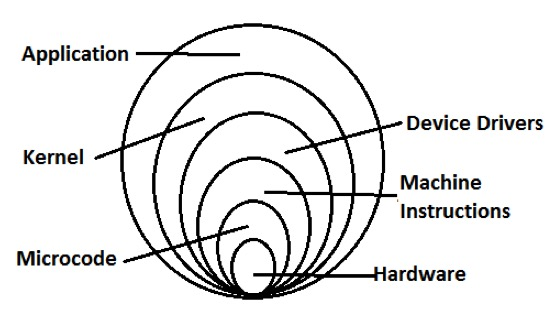
\includegraphics[scale=0.5]{m1/onionModel}
		\centering
\end{tcolorbox}

\begin{definition}{\textbf{Micro-coding}}
	CPU designers implement a set of basic operations directly in hardware, then create a ''microcode'' – a language – that uses these operations to create complex machine instructions. (\textbf{Reason}: some instructions are too complex to do properly in hardware (e.g. the Intel string and block operations).)
\end{definition}



\begin{tcolorbox}
	\textsf{Abstraction Layer \& Opearating System Structure}
	
	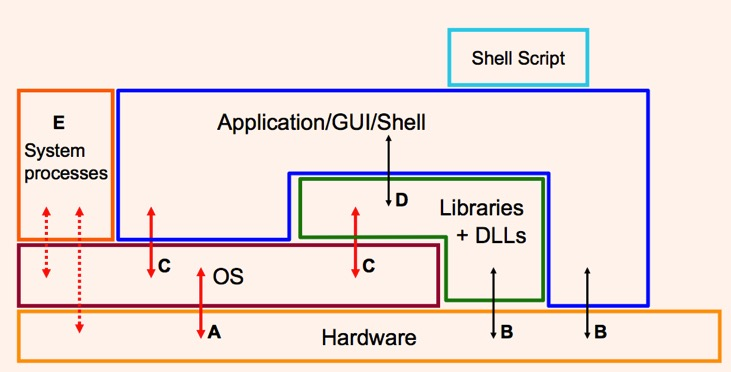
\includegraphics[scale=0.3]{m1/operatingSystemStructure}
		\centering
	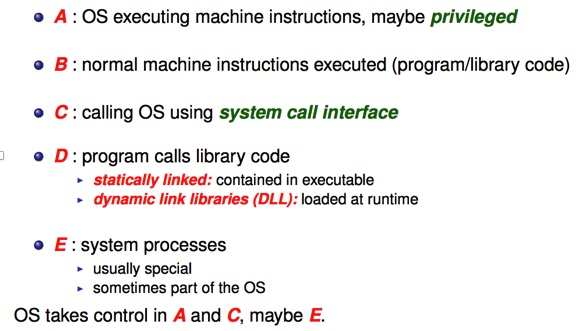
\includegraphics[scale=0.4]{m1/abstractionLayerDescription}
		\centering
\end{tcolorbox}

\begin{definition}{\textbf{Boostrapping}}
	\begin{myitemize}
	\item The \textbf{OS is not present in memory} when a system is “cold started”.
	\begin{myitemize}
		\item When a system is first started up, memory is completely empty.
	\end{myitemize}
	\item We start first with a \textbf{bootloader} to get an operating system into memory.
	\begin{myitemize}
	\item Tiny program in the first (few) sector(s) of the hard-disk.
	\item The first sector is generally called the “boot sector” or “master boot record” for this reason.
	\item Job is to load up the main part of the operating system and start it up.
	\end{myitemize}
\end{myitemize}
\end{definition}

\begin{definition}{\textbf{Core}}
	CPU units that can execute processes, because we have much more number of processes than the number of cores, we have to do \textbf{context switching} to share a core very quickly between different processes.
	\begin{myitemize}
		\item Entire sharing must be transparent.
		\item Processes can be suspended and resumed arbitrarily.
	\end{myitemize}
\end{definition}

\begin{definition}{\textbf{Context switching}}
	\begin{myenumerate}
		\item Save the \textsf{context} of the process to be suspended.
		\item Restore the \textsf{context} of the process to be (re)started.
		\item Issues of \textsf{scheduling} to decide which process to run.
	\end{myenumerate}
\end{definition}

\begin{definition}{\textbf{special register} Machine Status Word (MSW) or Status Register (SREG)}
\begin{figure}[!h]
	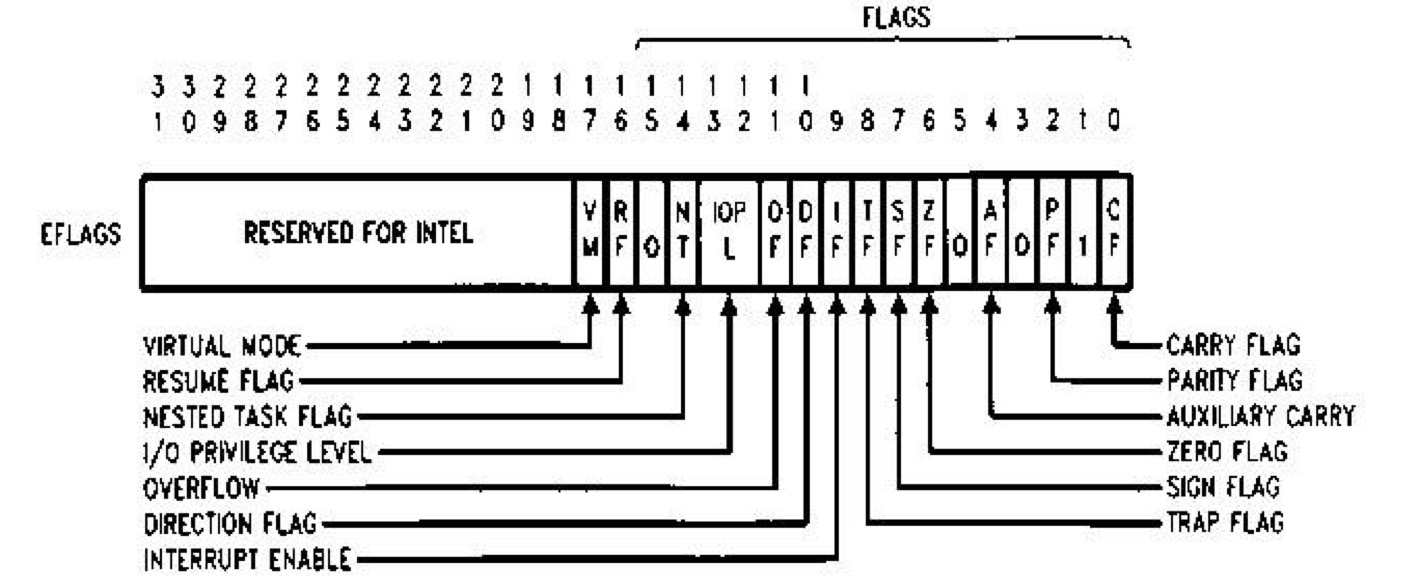
\includegraphics[scale=0.2]{m1/machineStatusWord}
	\centering
\end{figure}

	We can see that it contains flags that tell us the results of a previous arithmetic operation. E.g. Zero (ZF) tells us if a subtract resulted in a 0, Sign (SF) tells us if it resulted in a negative number. The Carry flag (CF) tells us if an addition resulted in a carry, the Overflow flag (OF) tells us if an overflow resulted (which means the results could be invalid), etc.
	
	The ZF and SF are necessary for branch instructions. E.g. for a branch on less than (BLT), the ALU performs a subtraction, and the branch is taken if SF is set. Similarly for a BEQ, the branch is taken if ZF is set, etc.
	
	The MSW also contains configuration flags, like the Interrupt Enable (IF) flag that enables or disables maskable interrupts (special signals that I/O hardware can use to get the CPU's attention – essentially this flag tells the CPU whether to entertain or ignore such requests).
	
	For correctness, MSW has to be stored during context save and restored during context restore.
\end{definition}

\begin{definition}{\textbf{File system}}
	A set of data structures on disk and within the OS kernel memory to organise persistent data.
\end{definition}

\begin{tcolorbox}
\textsf{How OS file system works?}

	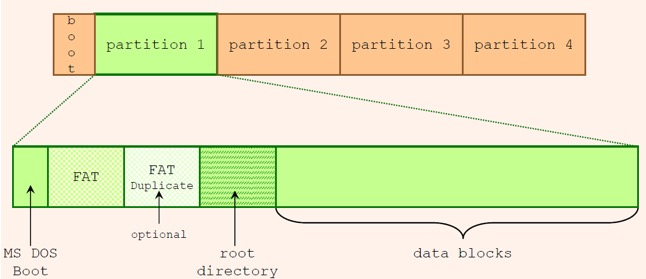
\includegraphics[scale=0.3]{m1/fileSystem}
	\centering
\end{tcolorbox}

\begin{tcolorbox}
	\textsf{Hardware Interfaces}
	
	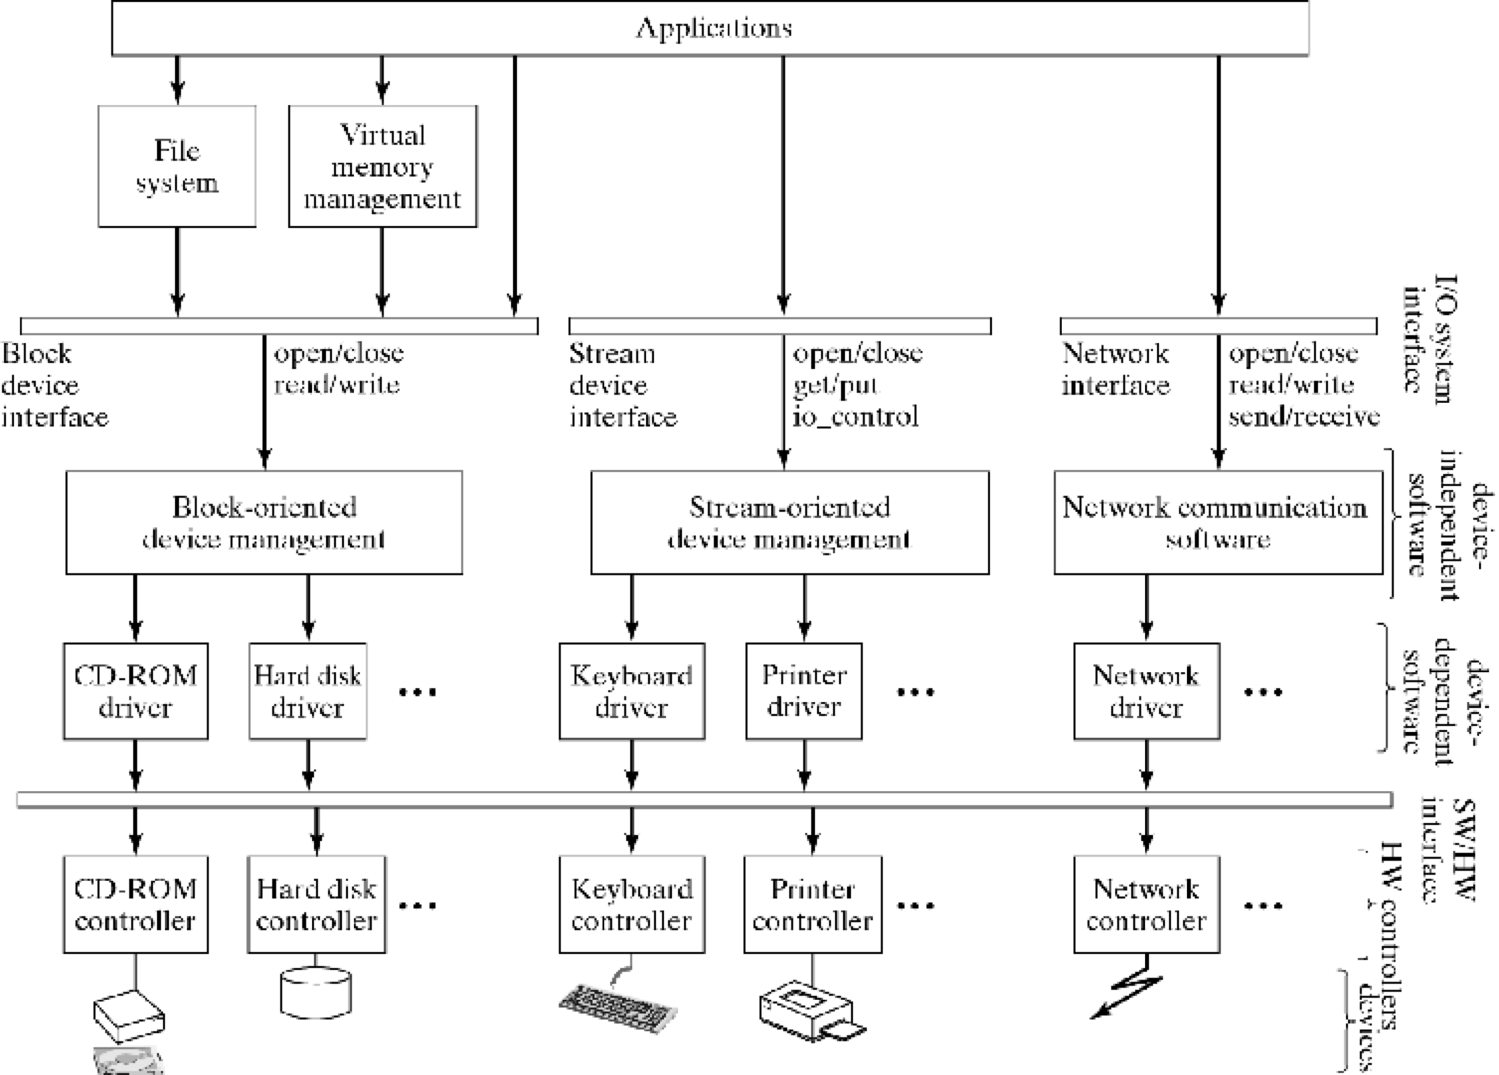
\includegraphics[scale=0.3]{m1/hardwareDevice}
	\centering
	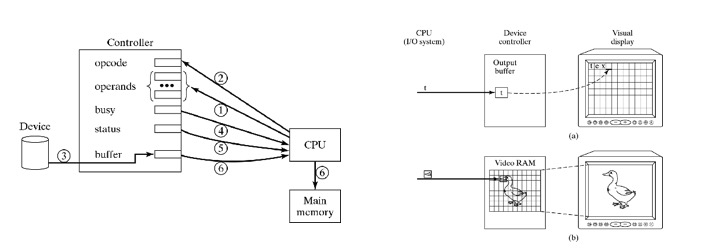
\includegraphics[scale=0.4]{m1/hardwareController}
	\centering
\end{tcolorbox}

\begin{definition}{\textbf{Memory}}
	static/dynamic (\textsf{new, delete, malloc, free}). Memory to store instructions
Memory to store data.
\end{definition}

\begin{tcolorbox}
	\textsf{Memory Management}
	
	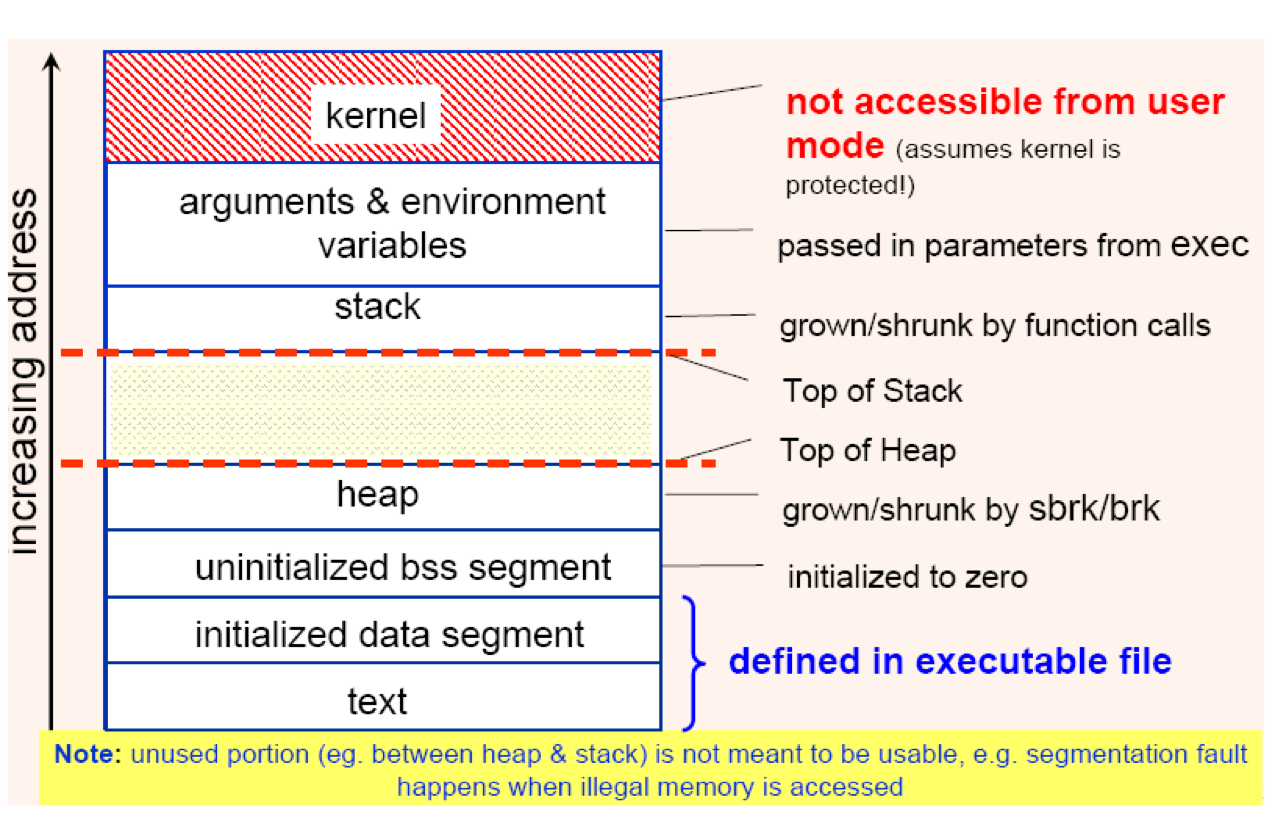
\includegraphics[scale=0.3]{m1/memoryManagement}
	\centering
\end{tcolorbox}

\begin{definition}{\textbf{Virtual Memory management}}
\begin{myitemize}
	\item For cost/speed reasons memory is organized in a hierarchy:
	\begin{figure}[h!]
		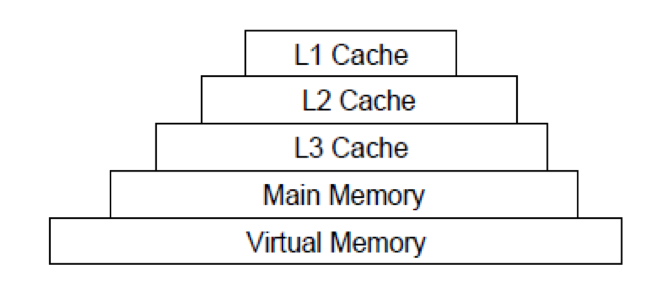
\includegraphics[scale=0.6]{m1/memoryHirarchy}
		\centering
	\end{figure}
	\item The lowest level is called ''virtual memory'' and is the slowest but cheapest memory.
	\begin{myitemize}
	\item Actually made using hard-disk space!
	\item Allows us to fit much more instructions and data than memory allows!
	\end{myitemize}
\end{myitemize}
\end{definition}

\begin{definition}{\textbf{OS security}}
	\begin{myitemize}
		\item Data (files): Encryption techniques, Access control lists
		\item Resources: Access to the hardware (biometric, passwords, etc), Memory access, File access, etc.
	\end{myitemize}
\end{definition}

\begin{tcolorbox}
	\textsf{Writing an OS (BSD Unix)}
	
	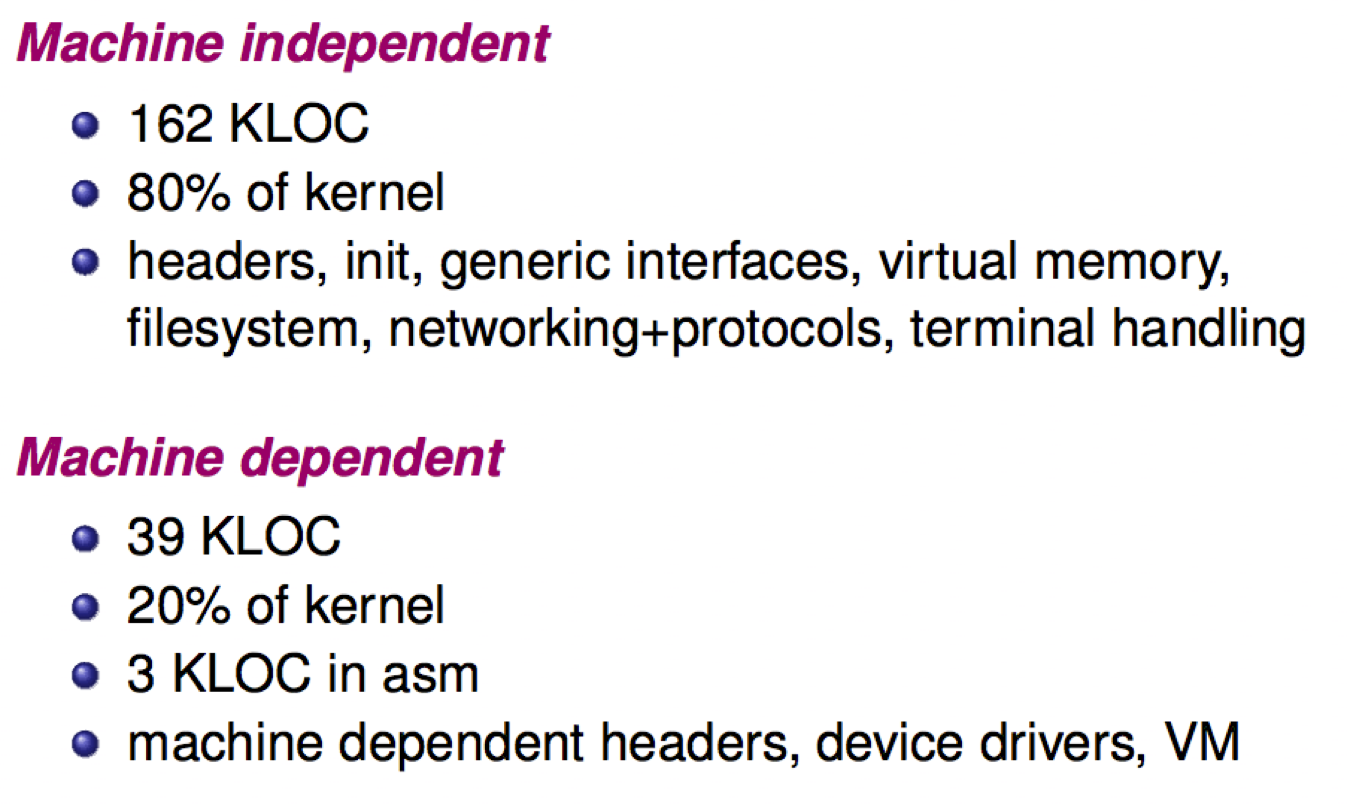
\includegraphics[scale=0.3]{m1/writingOS}
	\centering
\end{tcolorbox}

\begin{example}{\textbf{Privilege Levels}  used in Intel CPUs}
	
	This diagram is useful to understand privilege rings:
	
	\begin{figure}[!h]
		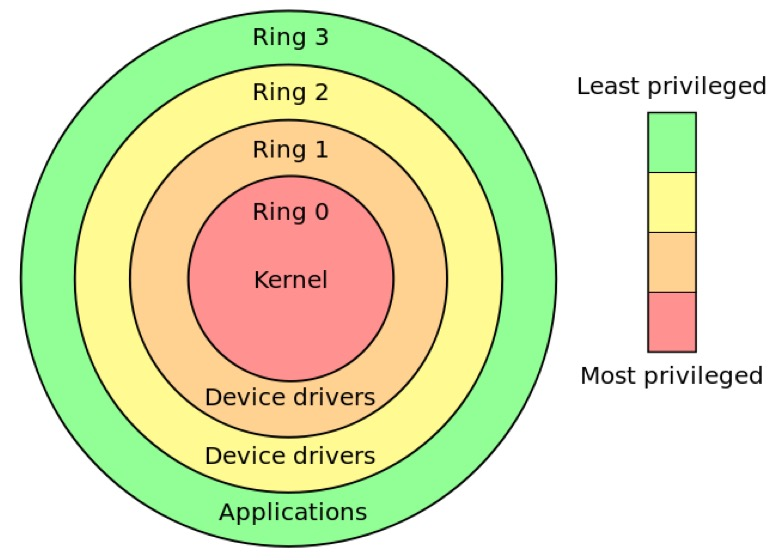
\includegraphics[scale=0.2]{m1/privilegeRing}
		\centering
	\end{figure}
	
	processes running in lower (outer) rings have more restrictive access to the machine than processes in the higher (inner) rings, to prevent a user, for example, from erasing the entire system drive.
	
	\begin{tcolorbox}
		\textsf{why the highest priority task can still be interrupted by the lowest priority interrupt}, and how this affects ISR design. (Hint: Interrupts are implemented in hardware in the CPU itself).
		
		This is because task priorities are seen only by the OS. As far as the CPU is concern, it is “just another program” that is running, with instructions being fetched and executed. On the other hand interrupt lines are checked at the end of each instruction execution cycle, so interrupts are always serviced regardless of their priority level (and of the priority level of the running task).
	\end{tcolorbox}
\end{example}

\begin{definition}{\textbf{Kernel}}
	\begin{myitemize}
		\item \textsf{Monolithic Kernel} (Linux, MS Windows)
		\begin{myitemize}
			\item All major parts of the OS-devices drivers, file systems, IPC, etc, running in ''kernel space'' (an elevated execution mode where certain privileged operations are allowed).
			\item Bits and pieces of the kernel can be loaded and unloaded at runtime (e.g. using ''modprobe'' in Linux)
			\begin{figure}[h!]
				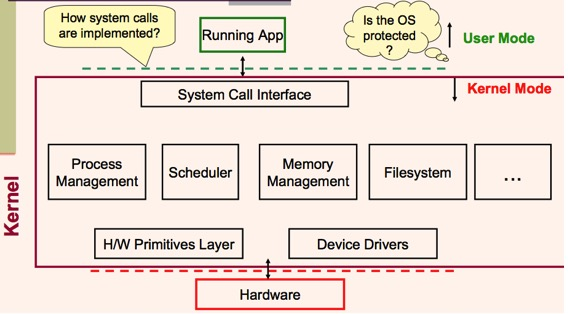
\includegraphics[scale=0.35]{m1/monolithicKernels}
				\centering
			\end{figure}
		\end{myitemize}
		\item \textsf{MicroKernel} (Mac OS)
		\begin{myitemize}
			\item Only the ''main'' part of the kernel is in ''kernel space'' (Contains the important stuff like the scheduler, process management, memory management, etc.)
			\item The other parts of the kernel operate in ''user space'' as system services: The file systems, USB device drivers, Other device drivers.
		\end{myitemize}
	\end{myitemize}
\end{definition}

\begin{tcolorbox}
	\textsf{External View of an OS}
	\begin{myitemize}
		\item The kernel itself is not very useful. (Provides key functionality, but need a way to access all this functionality.)
		\item We need other components:
		\begin{myitemize}
			\item System libraries (e.g. stdio, unistd, etc.)
			\item System services (creat, read, write, ioctl, sbrk, etc.)
			\item OS Configuration (task manager, setup, etc.)
			\item System programs (Xcode, vim, etc.)
			\item Shells (bash, X-Win, Windows GUI, etc.)
			\item Admin tools (User management, disk optimization, etc.)
			\item User applications (Word, Chrome, etc).
		\end{myitemize}
	\end{myitemize}
	
\end{tcolorbox}

\begin{definition}{\textbf{System Calls}}
	calls made to the “Application Program Interface” or API of the OS.
	\begin{myitemize}
		\item UNIX  and similar OS mostly follow the POSIX standard. (Based on C. Programs become more portable.) \textit{POSIX: portable operating system interface for UNIX, minimal set of system calls for application portability between variants of UNIX}.
		\item Windows follows the WinAPI standard. (Windows 7 and earlier provide Win32/Win64, based on C.
Windows 8 provide Win32/Win64 (based on C) and WinRT (based on C++).)
	\end{myitemize}
\end{definition}

\begin{example}{\textbf{User mode + Kernel mode}}
	\begin{myitemize}
		\item Programs (process) run in user mode.
		\item During system calls, running kernel code in kernel mode.
		\item After system call, back to user mode.
	\end{myitemize}
\end{example}

\begin{tcolorbox}
	\textsf{How to switch mode?} Use privilege mode to switching instructions:
	\begin{myitemize}
		\item syscall instruction
		\item software interrupt - instruction which raises specific interrupt from software.
	\end{myitemize}
\end{tcolorbox}

\begin{example}{\textbf{LINUX system call}}
	\begin{myitemize}
		\item User mode: (outside kernel)
		\begin{myitemize}
			\item C function wrapper (eg. \textbf{getpid()}) for every system call in C library.
			\item assembler code to setup the system call no, arguments
			\item trap to kernel	
		\end{myitemize}
		\item Kernel mode: (inside kernel)
		\begin{myitemize}
			\item dispatch to correct routine
			\item check arguments for errors (eg. invalid argument, invalid address, security violation)
			\item do requested service
			\item return from kernel trap to user mode
		\end{myitemize}
		\item User mode: (Outside kernel)
		\begin{myitemize}
			\item returns to C wrapper - check for error return values
		\end{myitemize}
	\end{myitemize}
\end{example}

\begin{example}{\textbf{UNIX signal}: SIGTERM or SIGKILL}
	\begin{myitemize}
		\item SIGTERM (triggered using \textsf{kill $<$process id$>$}):
		\begin{myitemize}
			\item The OS receives the SIGTERM request and passes it to the process.
			\item The process receives this signal and can clean up and release resources it is using.
			\item If the process has child processes, it will terminate the child processes also using a SIGTERM.
			\item The process exits gracefully.
		\end{myitemize}
		\item SIGKILL (triggered using \textsf{kill $-$9 $<$process id$>$}):
		\begin{myitemize}
			\item Process is terminated immediately by init (the UNIX master process). SIGKILL is not passed to the process, and the process does not have any chance to do cleaning up.
			\item SIGKILL can create zombie processes particularly if the killed process has children.
		\end{myitemize}
	\end{myitemize}
\end{example}

\section{Process Management}
\begin{definition}{\textbf{Program}}
	consists of: Machine instructions (and possibly source code) and Data. A program exists as a file on the disk. (e.g. command.exe, MSword.exe)
\end{definition}

\begin{definition}{\textbf{Process}}
	consists of Machine instructions (and possibly source code), Data and Context. It exists as instructions and data in memory, \textbf{may} be executing on the CPU.
\end{definition}

\begin{tcolorbox}
	\textsf{Program vs. Process}
	
	A single program can produce multiple processes. (e.g. chrome.exe is a single program, but every tab in Chrome is a new process!)

\end{tcolorbox}

\begin{definition}{\textbf{Execution Modes}}
	\begin{myitemize}
		\item Programs usually run sequentially. (Each instruction is executed one after the other.)
		\item Having multiple cores or CPUs allow parallel (''concurrent'') execution. (Streams of instructions with no dependencies are allowed to execute together.)
		\item A multitasking OS allows several programs to run ''concurrently''. (Interleaving, or “time-slicing”)
	\end{myitemize}
\end{definition}

\begin{remark}
	we mostly assume number of processes $\geq$ number of CPU otherwise can have idle tasks. So each core must still switch between processes even for multi-cores, and we will assume a single processor with a single core.
\end{remark}

\begin{tcolorbox}
	\textsf{The Process Model}
	
	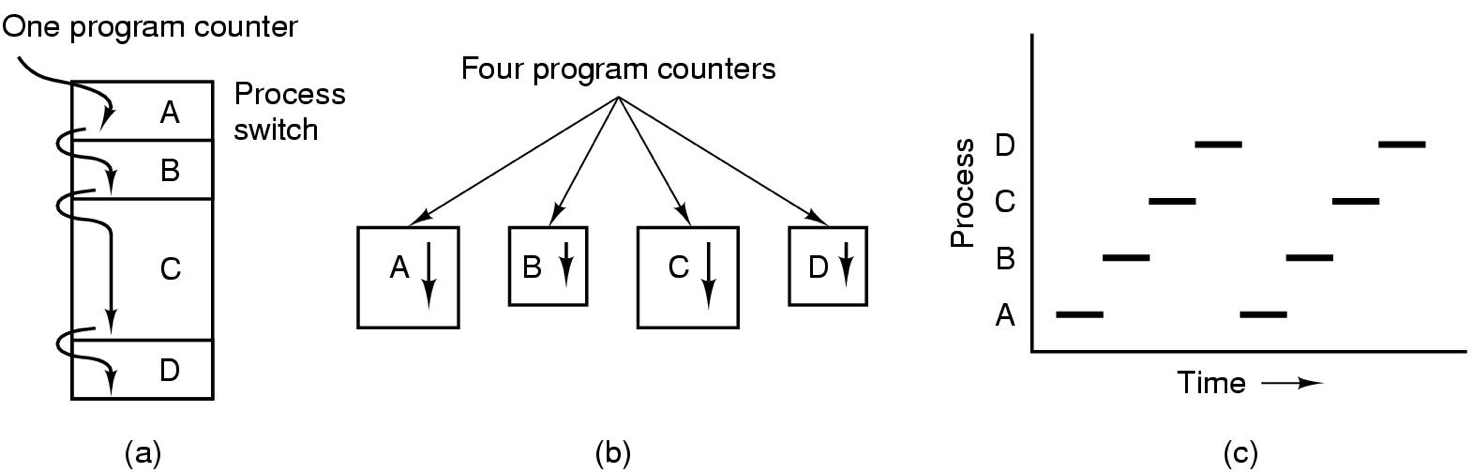
\includegraphics[scale=0.5]{m1/processModel}
	\centering
	
	\begin{myitemize}
		\item Figure (b) shows what “appears” to be happening in a single processor system running multiple processes:
		\begin{myitemize}
			\item There are 4 processes each with its own program counter (PC) and registers.
			\item All 4 processes run independently of each other at the same time.
		\end{myitemize}
		\item Figure (a) shows what actually happens.
		\begin{myitemize}
			\item There is only a single PC and a single set of registers.
			\item When one process ends, there is a ''context switch'' or ''process switch'':
			\begin{myitemize}
				\item PC, all registers and other process data for Process A is copied to memory.
				\item PC, register and process data for Process B is loaded and B starts executing, etc.
			\end{myitemize}
		\end{myitemize}
		\item Figure (c) illustrates how processes A to D share CPU time.
	\end{myitemize}
\end{tcolorbox}

\begin{definition}{\textbf{Process States}} there are three possible states for a process
	\begin{myitemize}
		\item Running 
		\begin{myitemize}
			\item The process is actually being executed on the CPU.
		\end{myitemize}
		\item Ready 
		\begin{myitemize}
			\item The process is ready to run but not currently running. 
			\item A ''scheduling algorithm'' is used to pick the next process for running.
		\end{myitemize}
		\item Blocked.
		\begin{myitemize}
			\item The process is waiting for ''something'' to happen so it is not ready to run yet. e.g. include waiting for inputs from another process.
		\end{myitemize}
	\end{myitemize}
\end{definition}

\begin{figure}[h!]
	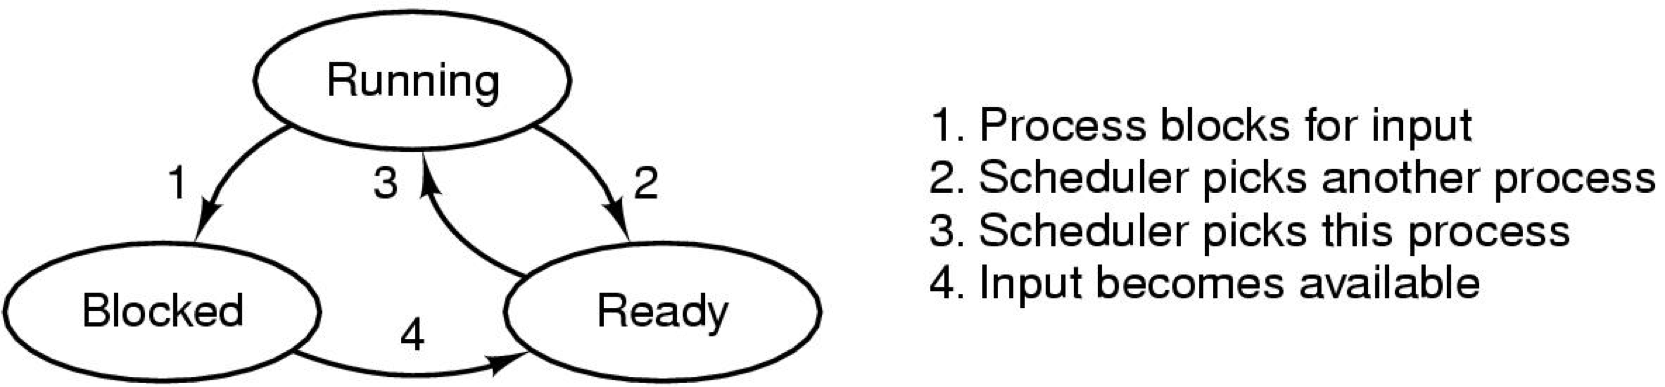
\includegraphics[scale=0.3]{m1/processStates}
	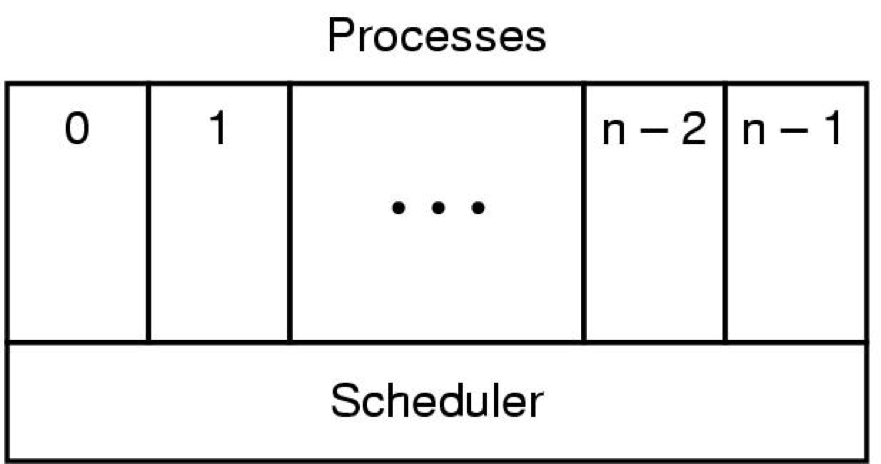
\includegraphics[scale=0.3]{m1/processStates2}
	\centering
\end{figure}

\begin{definition}{\textbf{Process Context}} (values change as a process runs)
	\begin{myitemize}
		\item CPU register values. 
		\item Stack pointers.
		\item CPU Status Word Register
		\begin{myitemize}
			\item This maintains information about whether the previous instruction resulted in an overflow or a ''zero'', whether interrupts are enabled, etc.
			\item This is needed for branch instructions – assembly equivalents of ''if'' statements.
		\end{myitemize}
	\end{myitemize}
\end{definition}

\begin{figure}[h!]
	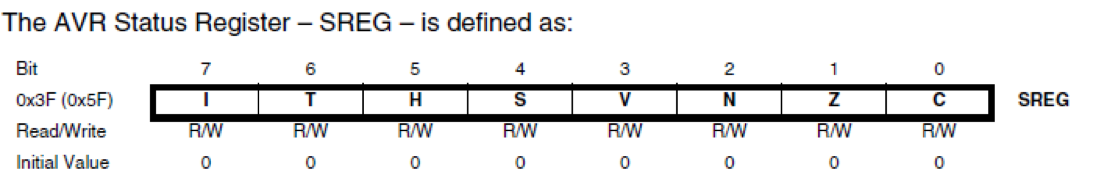
\includegraphics[scale=0.6]{m1/statusRegister}
	\centering
\end{figure}

\begin{tcolorbox}
	\textsf{What other pieces of information does the OS need to save about a process?}
	
	\begin{myitemize}
		\item \textbf{File handles / Open File Table}: These are data structures that maintain information about files that are opened by the process, like the location that a process is inside the file, access rights to the file, file open modes, etc.
		\item \textbf{Pending signals}: A “signal” is an OS message to the process.
		\item \textbf{Process Running State}: Whether the process is suspending, ready, running, terminated, etc.
		\item \textbf{Accounting Information}: How much CPU time the process has used, how much disk space, network activity, etc.
		\item \textbf{Process ID}: Unique number identifying the process. Etc.
	\end{myitemize}
\end{tcolorbox}

\begin{example}{\textbf{Context Switching in FreeRTOS Atmega Port}}
	FreeRTOS relies on regular interrupts from Timer 0 to switch between tasks. When the interrupt triggers:
	\begin{myenumerate}
		\item PC is placed onto Task A’s stack.
		\item The ISR calls \textsf{portSAVECONTEXT}, resulting in Task A’s context being pushed onto the stack.
		\item \textsf{pxCurrentTCB} will also hold SPH/SPL after the context save.
		\begin{myitemize}
			\item This must be saved by the kernel.
			\item The kernel stores a copy of the stack pointer for each task.
		\end{myitemize}
		\item The kernel then selects Task B to run, and copies its SPH/SPL values into \textsf{pxCurrentTCB} and calls \textsf{portRESTORE\_CONTEXT}.
		\item The rest of \textsf{portRESTORE\_CONTEXT} is executed, causing Task B’s data to be loaded into R31-R0 and SREG. Now Task B can resume like as though nothing happened
		\item Only Task B’s PC remains on the stack. Now the ISR exits, causing this value to be popped off onto the AVR’s PC.
		\begin{myitemize}
			\item PC points to the next instruction to be executed. 
			\item End result: Task B resumes execution, with all its data and SREG intact!
		\end{myitemize}
	\end{myenumerate}
\end{example}

\begin{tcolorbox}
	\textsf{How can context switching be triggered?}
	
	It can be triggered by a timer; currently running process waiting for input; currently running task blocking on a synchronisation mechanism; currently running task wants to sleep for a fixed period; higher priority task becoming “READY”; $\dots$
\end{tcolorbox}

\begin{definition}{\textbf{Process Control Block}}
	maintains information about that process: Process ID (PID), Stack Pointer, Open files, Pending signals, CPU usage, $\dots$
\end{definition}

\begin{tcolorbox}
	\textsf{Process Life Cycle}
	
	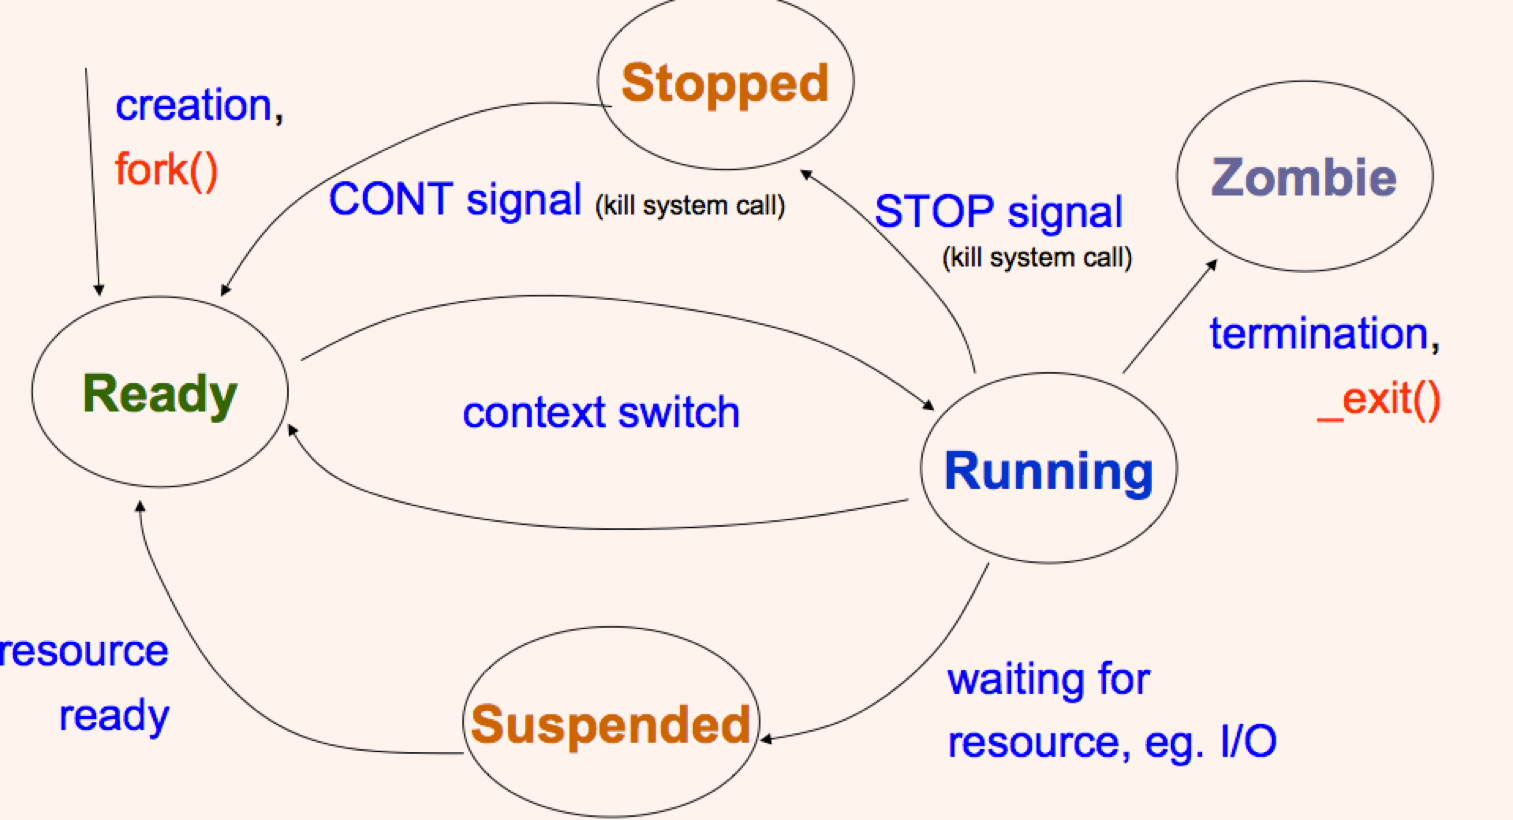
\includegraphics[scale=0.3]{m1/processLifeCycle}
	\centering
\end{tcolorbox}

\begin{definition}{\textbf{Creating a new process - \textsf{fork()}}}
	\begin{myitemize}
		\item Fork system call creates a new process by duplicating the current image into a new process, \textit{child process}
		\item \textsf{same code} (executable image) is executed
		\item Child differs only in process id (PID) and parent (PPID), fork return value
		\item Data in child is a COPY of the parent (i.e. not shared)
		\item In PARENT process after fork:
		\begin{myitemize}
			\item PC is at return from fork system call
			\item fork return value: new child PID
		\end{myitemize}
		\item In CHILD process after fork:
		\begin{myitemize}
			\item PC is at return from fork system call
			\item fork return value: 0
			\item Shares open file \& signal handlers with parent, current working directory
			\item Independent copy of: memory, arguments, environment variables (note: cloning example)
		\end{myitemize}
		\item fork return result is -1 if the fork failed.
		\item \textsf{for(int i=0; i$<$10; i++) fork();}, this for general case n, there are $2^n$ processes created including the original process. 
	\end{myitemize}
\end{definition}

\begin{definition}{\textbf{The Master Process}}
	\begin{myitemize}
		\item Every process has parent: \textsf{where does it stop?}
		\item Special initial process - \textsf{init} process created in kernel at the end UNIX boot process, traditionally having PID=1.
		\item Forking creates process tree, \textsf{init} is the root process.
		\item \textsf{init} watches for processes and response where needed, e.g. terminal login.
		\item \textsf{init} also manages system run levels (e.g. shutdown, power failure, single-user mode), etc. Example of a system-like process running in kernel mode.
	\end{myitemize}
\end{definition}

\begin{definition}{\textbf{Start/Stop a Process}}
	\begin{myitemize}
		\item kill() system call sends signal to process
		\item Special process signals:
		\begin{myitemize}
			\item stopping process (SIGSTOP)
			\item killing process (SIGKILL)
			\item restart stopped process (SIGCONT)
		\end{myitemize}
	\end{myitemize}
\end{definition}

\begin{tcolorbox}
	\textsf{Terminating a process}
	
	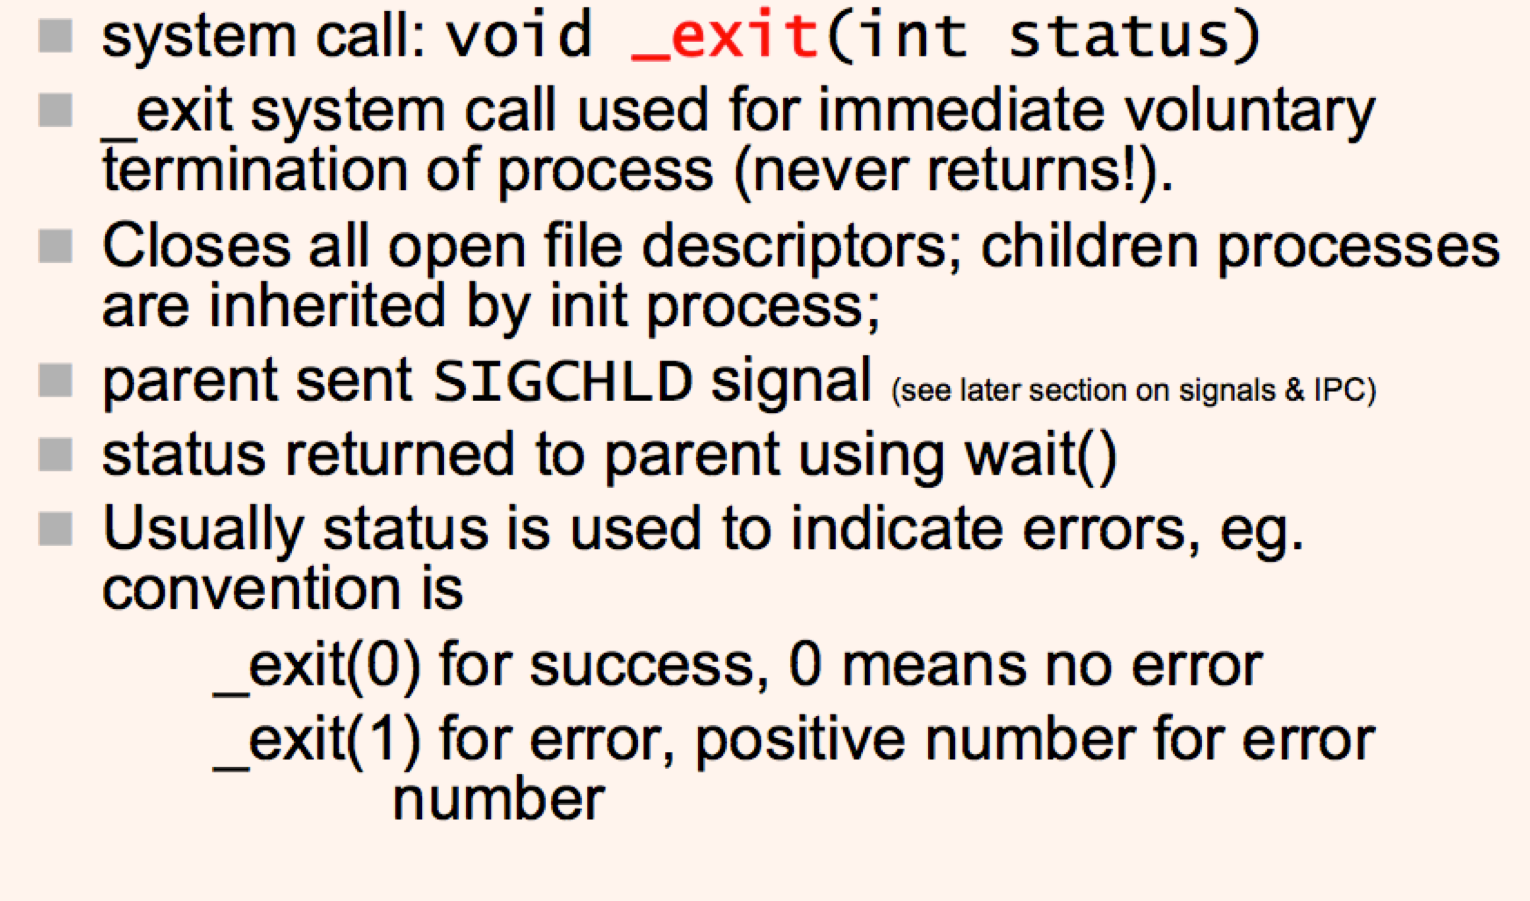
\includegraphics[scale=0.33]{m1/terminatingProcess1}
	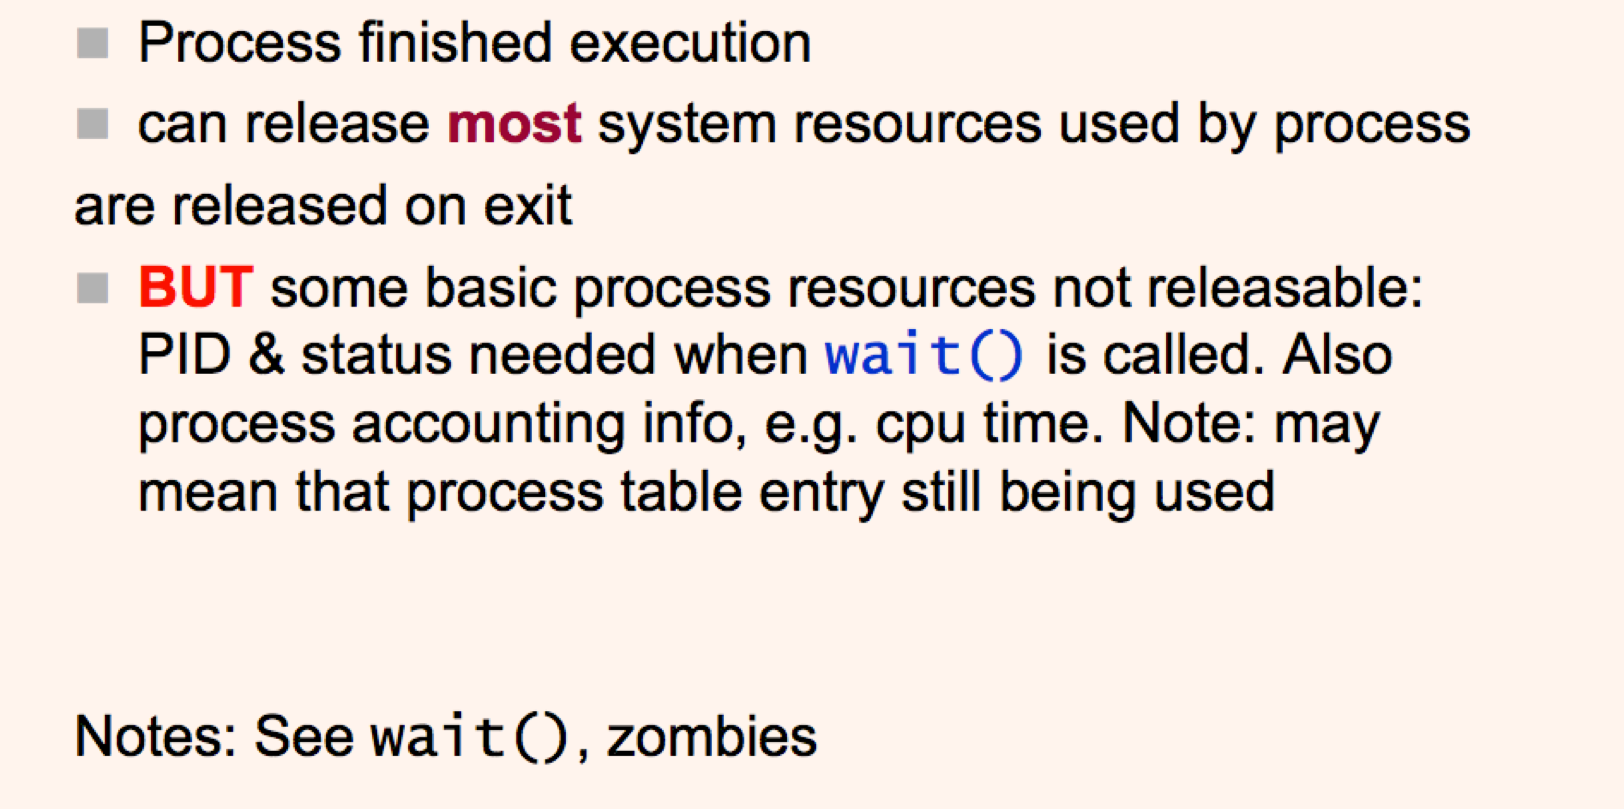
\includegraphics[scale=0.33]{m1/terminatingProcess2}
	\centering
\end{tcolorbox}

\begin{definition}{\textbf{Normal Program Termination} - \textsf{void exit(int status)} from standard C library function}
	\begin{myitemize}
		\item Usuall don't use \textsf{\_exit()} but \textsf{exit()}, which cleans up: open streams from C stdio library (e.g., fopen, printf) are flushed and closed
		\item calls some exit handlers
		\item finally calls \textsf{\_exit(status)} after all standard C cleanup done.
	\end{myitemize}
\end{definition}
\begin{remark}
	returning from \textsf{main()} implicitly calls exit. \textsf{exec} didn't actually call main directly but a startup routine. Open files also get flushed automatically.
\end{remark}

\begin{tcolorbox}
	\textsf{Waiting for Child Processes to Terminate - process interaction}
	
	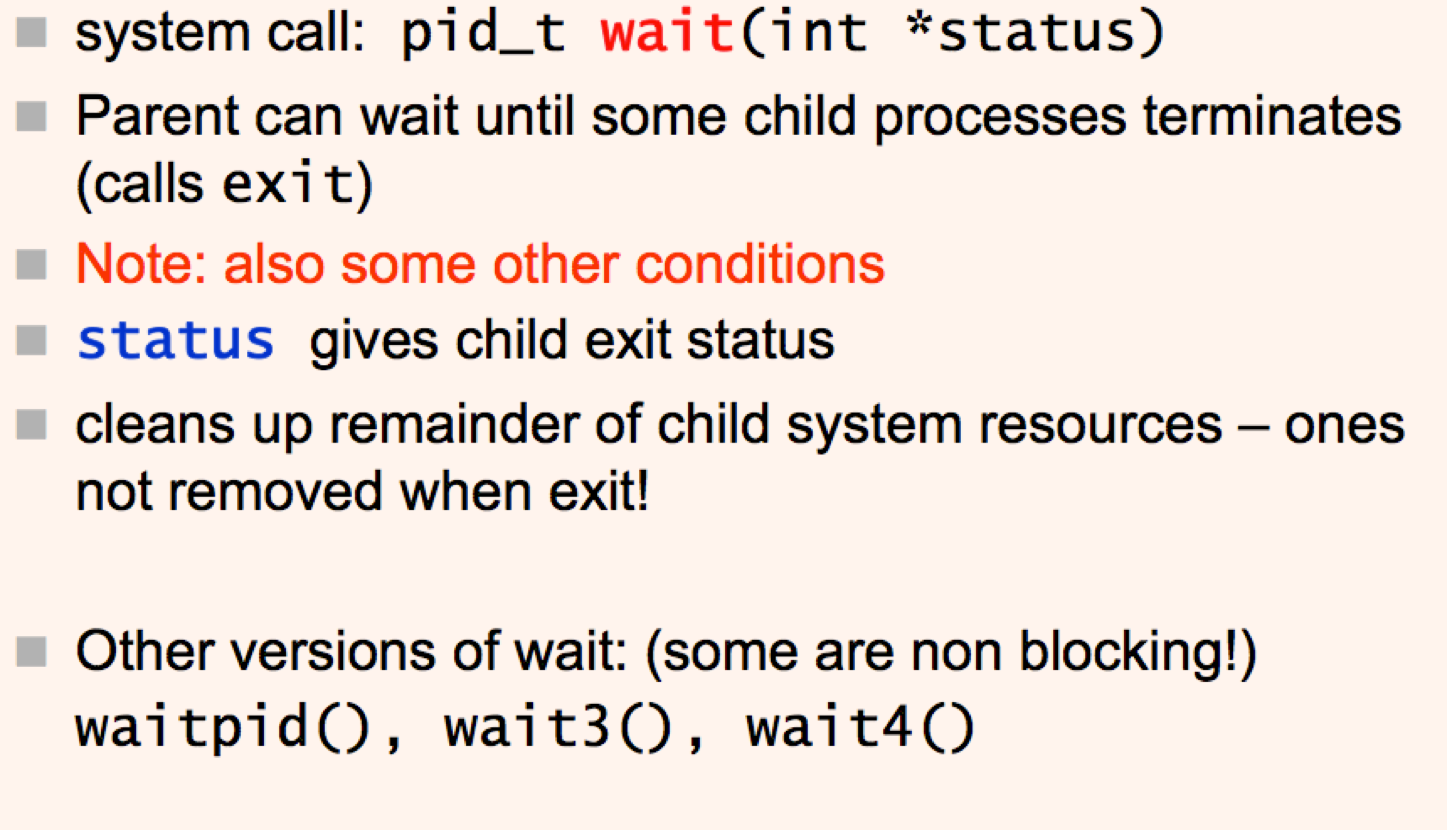
\includegraphics[scale=0.33]{m1/parentWait1}
	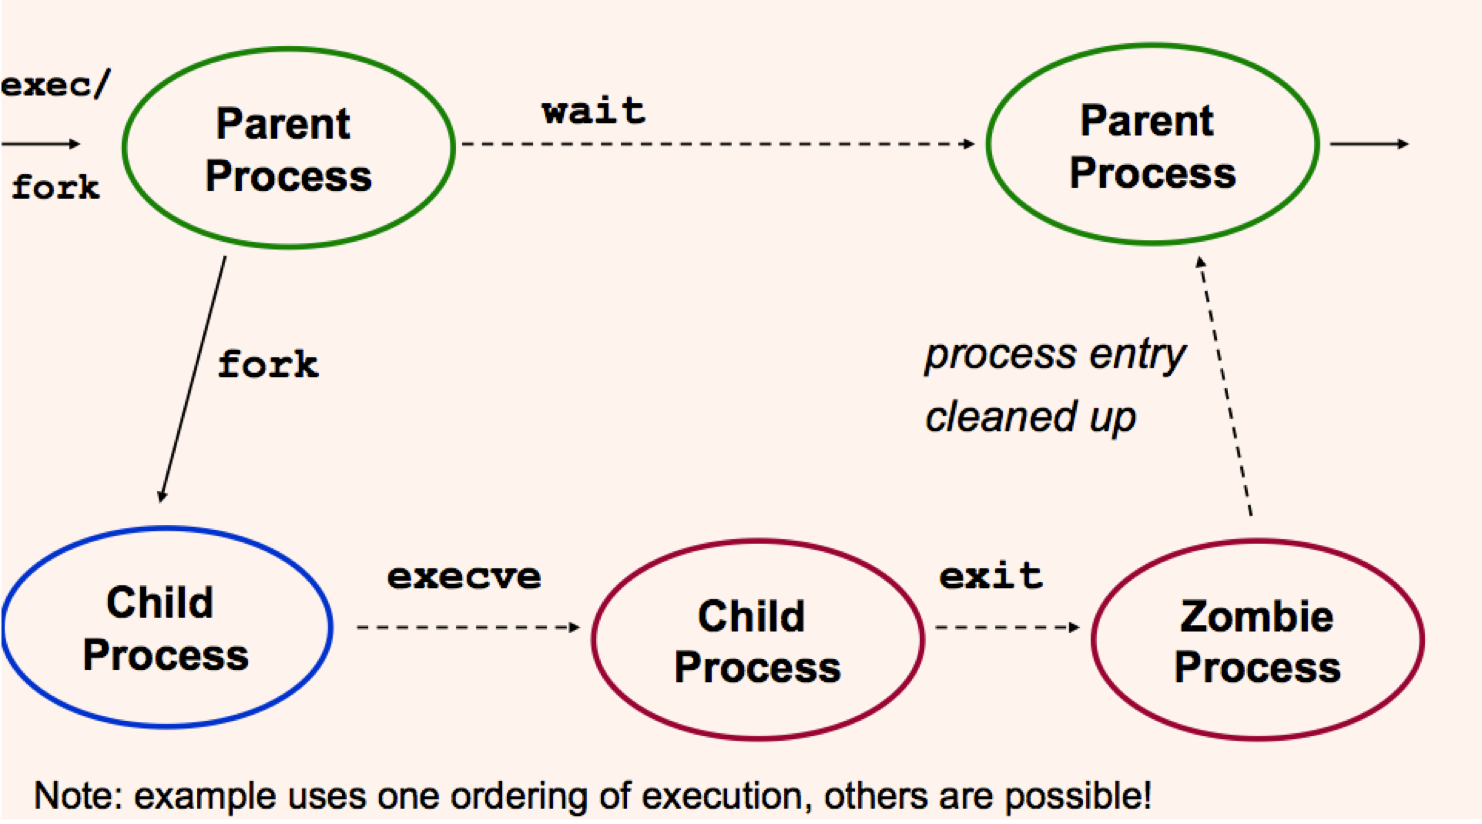
\includegraphics[scale=0.33]{m1/parentWait2}
	\centering
\end{tcolorbox}

\begin{tcolorbox}
	\textsf{Zombie Process}
	
	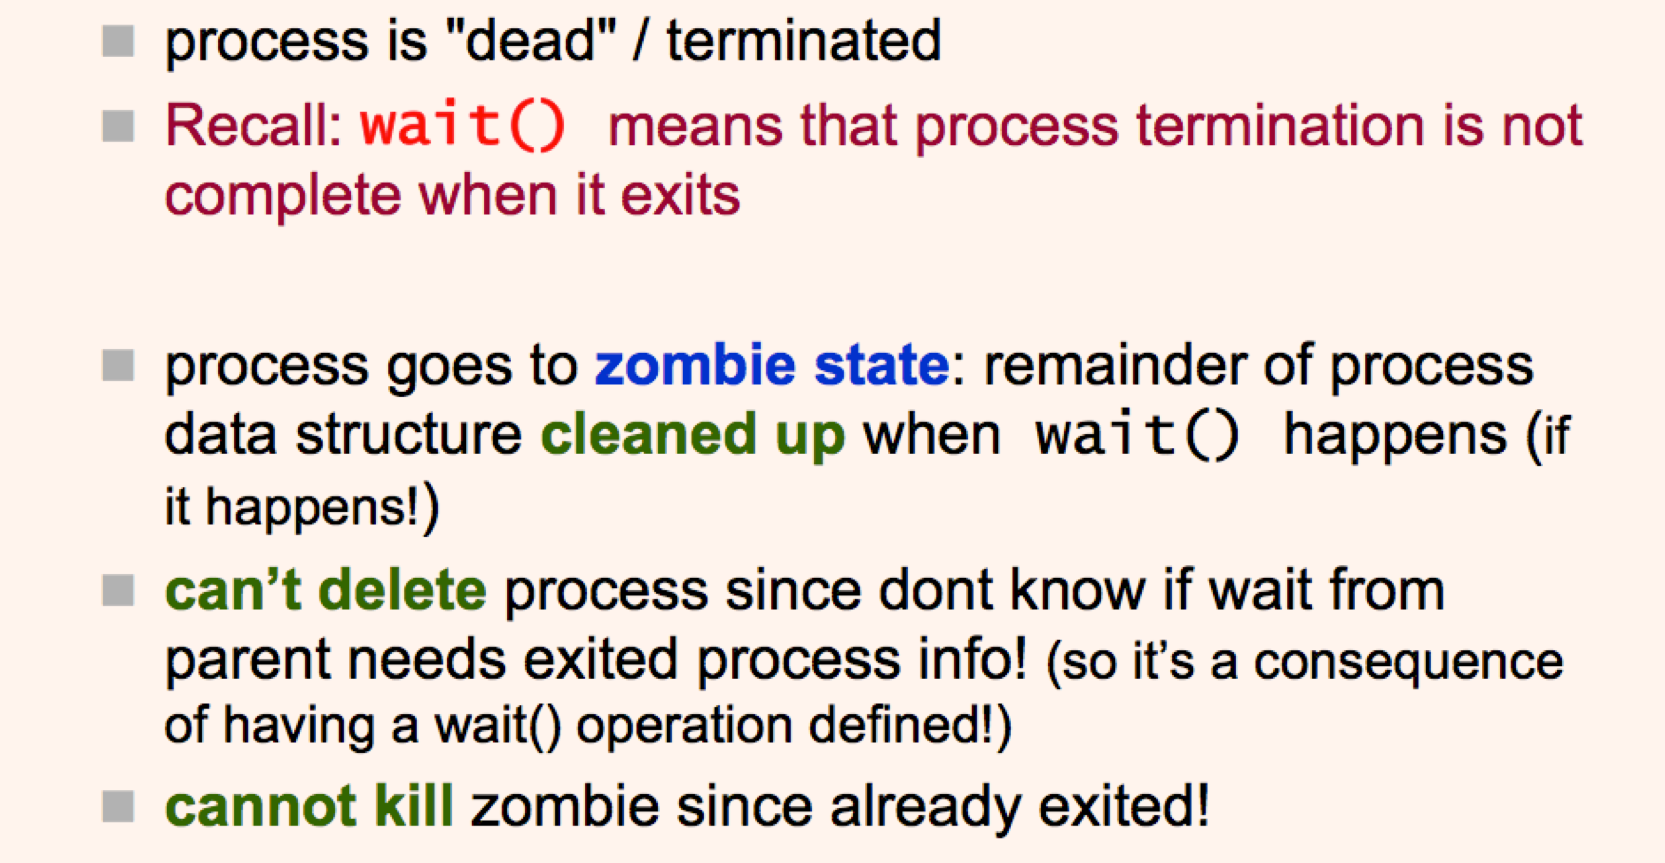
\includegraphics[scale=0.30]{m1/zombieProcess1}
	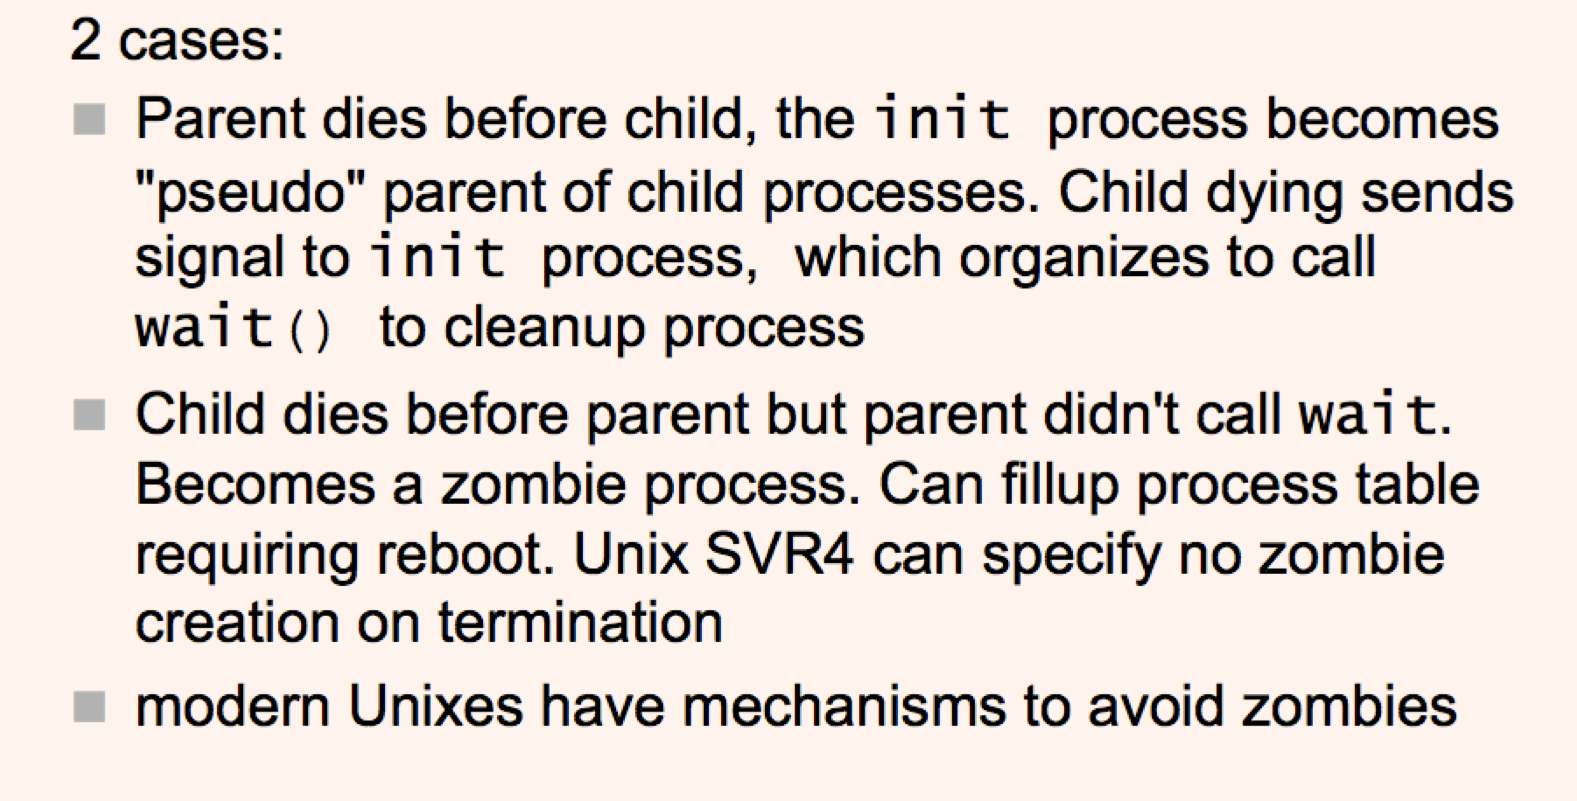
\includegraphics[scale=0.30]{m1/zombieProcess2}
	\centering
\end{tcolorbox}

\section{Process Scheduling}

\begin{definition}{\textbf{Computer jobs}}
	Computatings + reading/writing memory + input/output.
	\begin{myitemize}
		\item CPU bound
		\begin{myitemize}
			\item Most of the time spent on processing on CPU
			\item Graphics-intensive applications are considered to be ''CPU'' bound.
			\item Multitasking opportunities come from having to wait for processing results.
		\end{myitemize}
		\item I/O bound
		\begin{myitemize}
			\item Most of the time is spent on communicating with I/O devices
			\item Multitasking opportunities come from having to wait for data from I/O devices.
		\end{myitemize}
	\end{myitemize}
\end{definition}

\begin{tcolorbox}
	\textsf{Process states - scheduler involvement}
	
	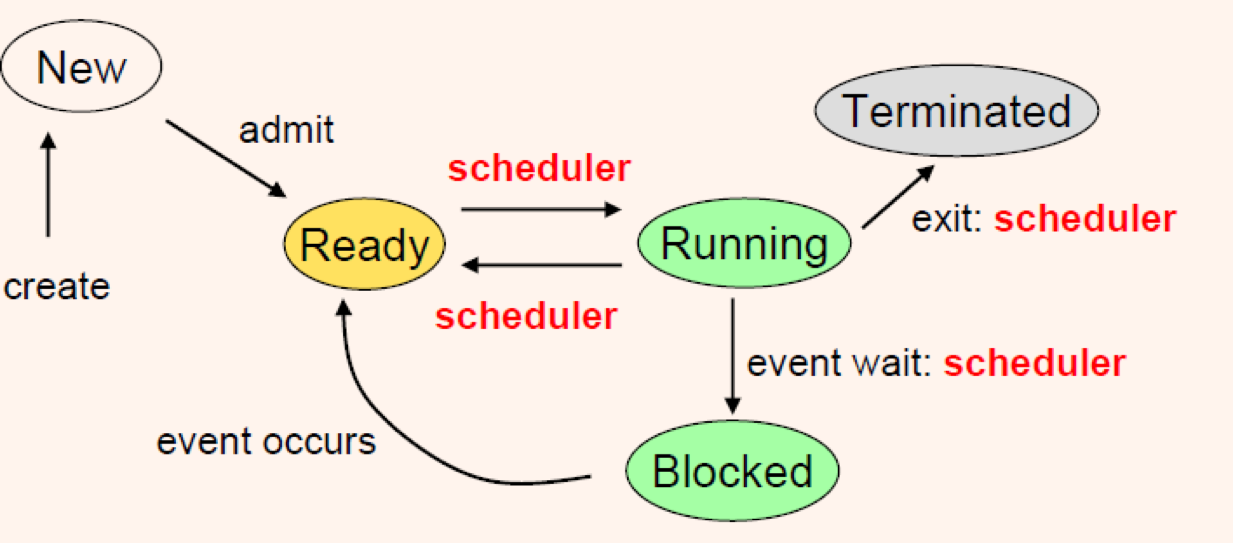
\includegraphics[scale=0.4]{m1/processSchedulerStates}
	\centering
\end{tcolorbox}

\begin{definition}{\textbf{Types of Multitaskers}}
	\begin{myitemize}
		\item Batch Processing (Not actually multitasking since only one process runs at a time to completion.)
		\item Co-operative Multitasking (Currently running processes cannot be suspended by the scheduler; Processes must volunteer to give up CPU time. Context switching is controlled entirely by processes themselves. Co-operative multitasking is simpler and less prone to concurrency issues, but should any process go into an infinite loop, it could potentially freeze up the system.)
		\item Pre-emptive Multitasking (Currently running processes can be forcefully suspended by the scheduler. \textsf{Timer-triggered} multitasking.)
		\item Real-Time Multitasking (Processes have fixed deadlines that must be met.)
		\begin{myitemize}
			\item Hard Real Time Systems: Disaster strikes! System fails, possibly catastrophically!
			\item Soft Real Time Systems: Mostly just an inconvenience. Performance of system is degraded
		\end{myitemize}
	\end{myitemize}
\end{definition}
\begin{remark}
	Policies are determined by the kind of multitasking environment.
\end{remark}

\begin{method}{\textbf{Scheduling Policies} - enforce a priority ordering over processes}
	\begin{myitemize}
		\item \textbf{Fixed Priority} for all kinds of multitaskers
		\begin{myitemize}
			\item Each task is assigned a priority by the programmer. (usually priority number 0 has the highest priority.)
			\item Tasks are queued according to priority number.
			\item Batch, Co-operative: Task with highest priority is picked to be run next.
			\item Pre-emptive, Real-Time: When a higher priority task becomes ready, current task is suspended and higher priority task is run.
		\end{myitemize}
		\item Policies for \textbf{Batch Processing}
		\begin{myitemize}
			\item First-come First Served (\textsf{FCFS})
			\begin{myitemize}
				\item Arriving jobs are stored in a queue.
				\item Jobs are removed in turn and run.
				\item Particularly suited for batch systems.
				\item Extension for interactive systems: Jobs removed for running are put back into the back of the queue. This is also known as “round-robin scheduling”.
				\item Starvation free as long as earlier jobs are bounded.
			\end{myitemize}
			\item Shortest Job First (\textsf{SJF})
			\begin{myitemize}
				\item Processes are ordered by total CPU time used.
				\item Jobs that run for less time will run first.
				\item Reduces average waiting time if number of processes is fixed.
				\item Potential for starvation.
			\end{myitemize}
		\end{myitemize}
		\item Policies for \textbf{Co-operative Multitasking}
		\begin{myitemize}
			\item Round Robin with Voluntary Scheduling (\textsf{VS})
			\item \textbf{Voluntary Scheduling}: Processes call a special “yield” function. This invokes the scheduler. Causes the process to be suspended and another process started up.
		\end{myitemize}
		\item Policies for \textbf{Pre-emptive multitasking}
		\begin{myitemize}
			\item Round Robin with Timer (\textsf{RR})
			\begin{myitemize}
				\item Each process is given a fixed time slot $c_i$.
				\item After time $c_i$, scheduler is invoked and next task is selected on a round-robin basis.
			\end{myitemize}
			\item Shortest Remaining Time (\textsf{SRT})
			\begin{myitemize}
				\item Pre-emptive form of SJF.
				\item Processes are ordered according to remaining CPU time left.
			\end{myitemize}
		\end{myitemize}
		\item Policies for \textbf{Real-Time Multitaskers}
		\begin{myitemize}
			\item Rate Monotonic Scheduling (\textsf{RMS})
			\begin{myitemize}
				\item Processes are prioritized according to $P_i$, Shortest period = highest priority.
				\item \textbf{Critical Instance Analysis} is used to test that all processes meet their deadlines
			\end{myitemize}
			\item Earliest Deadline First Scheduling (\textsf{EDF})
			\begin{myitemize}
				\item Processes are prioritized according to who is closest to their respect deadlines.
				\item All processes are guaranteed to meet their deadlines as long as: $U=\sum^n_{i=1}\dfrac{C_i}{T_i} \leq 1$
				\item There is no context switching for processes, each process will run till the end if gets started.
			\end{myitemize}
		\end{myitemize}
	\end{myitemize}
\end{method}

\begin{remark}{\textbf{Real Time Scheduling}}
	must guarantee that processes complete within time limits.
	
	\begin{myitemize}
		\item Time limits are called “deadlines”
		\item Processes are assumed to be periodic with period $P_i$ for process i.
		\item Processes are assumed to use a fixed amount of CPU time $C_i$ each time.
		\item Deadline $D_i$ is assumed to be the same as period $P_i$. (if a process runs at time $T_i$, it must finish running by $D_i=T_i+P_i$, If it doesn’t, process has missed its deadline.) $T_i$ is the process or task arriving time.
	\end{myitemize}
\end{remark}

\begin{method}{\textbf{Critical Instance Analysis for} \textsf{RMS}}
	\begin{myenumerate}
		\item Sort T by period of each task, if T is not already sorted. (We will assume that $T_1$ has the shortest period, $T_2$ has the $2^{nd}$ shortest, etc.)
		\item For each task $T_i \in T$, recursively compute $S_{i0}, S_{i1}, \dots$ where:
		\[ S_{i,0}=\sum^i_{j=1}C_j; S_{i,(x+1)}=C_i+\sum^{i-1}_{j=1}C_j\times \ceil{\frac{S_{i,x}}{P_j}}  \]
		\item Stop when $S_{i,(x+1)}=S_{i,x}$. Call this $S_{i,(x+1)}$ the final value $S_{i,F}$ (termination value).
		\item If $S_{i,F}<D_i (=T_i+P_i)$, then the task i is schedulable and will not miss its deadlines.
	\end{myenumerate}
\end{method}

\begin{method}{\textbf{Managing Multiple Policies}}
	Multiple policies can be implemented on the same machine using multiple queues:
	\begin{myitemize}
		\item Each queue can have its own policy.
		\item This scheme is used in Linux, as we will see shortly.
	\end{myitemize}
\end{method}

\begin{example}{\textbf{Scheduling in Linux}}
	\begin{myitemize}
		\item Processes in Linux are dynamic:
		\begin{myitemize}
			\item New processes can be created with \textsf{fork()}
			\item Existing processes can exit.
		\end{myitemize}
		\item Priorities are also dynamic:
		\begin{myitemize}
			\item Users and superusers can change priorities using ''nice'' values.
			\item \textsf{nice –n 19 tar cvzf archive.tgz *} (Allows tar to run with a priority lowered by 19 to reduce CPU load. Normal users can only $0\leq n \leq 19$. Superusers can specify $-20\leq n \leq 19$. Negative nice increases priority.)
		\end{myitemize}
		\item Linux maintains \textbf{three types of processes}:
		\begin{myitemize}
			\item \textbf{Real-time FIFO}: \textsf{RT-FIFO} processes cannot be pre-empted except by a higher priority \textsf{RT-FIFO} process.
			\item \textbf{Real-time Round-Robin}: Like \textsf{RT-FIFO} but processes are pre-empted after a time slice.
			\item Linux only has ''soft real-time'' scheduling. (Priority levels 0 to 99) Cannot guarantee deadlines, unlike \textsf{RMS} and \textsf{EDF}. 
			\item Non-real time processes (Priority levels 100 to 139)
		\end{myitemize}
		\item Linux maintains 280 queues in two sets of 140: An active set, an expired set.
		\item The scheduler is called at a rate of 1000 Hz. (e.g. time tick is 1 ms, called a ''jiffy''.) \textsf{RT-FIFO} processes are \textbf{always} run if any are available. Otherwise:
		\begin{myitemize}
			\item Scheduler picks highest priority process in active set to run.
			\item When its “time quantum” is expired, it is moved to the expired set. Next highest priority process is picked.
			\item When active set is empty, active and expired pointers are swapped. Active set becomes expired set and vice versa.
			\item Scheme ensures no starvation of lowest priority processes.
		\end{myitemize}
		\begin{tcolorbox}
			\textsf{What happens if a process becomes blocked? (e.g. on I/O)}
			
			\begin{myitemize}
				\item CPU time used so far is recorded. Process is moved to a queue of blocked processes.
				\item When process becomes runnable again, it continues running until its time quantum is expired.
				\item It is then moved to the expired set.
				\item When a process becomes blocked its priority is often upgraded (see later). 
			\end{myitemize}
		\end{tcolorbox}
		\item Time quantums for RR processes: Varies by priority. For example: Priority level 100 – 800 ms, Priority level 139 – 5 ms, System load
		\item How process priorities are calculated: Priority = base + f(nice) + g(cpu usage estimate)
		\begin{myitemize}
			\item $f(.) =$ priority adjustment from nice value.
			\item $g(.) =$ Decay function. Processes that have already consumed a lot of CPU time are downgraded.
			\item Other heuristics are used: Age of process, More priority for processes waiting for I/O - I/O boost, Bias towards foreground tasks.
		\end{myitemize}
		\item \textbf{I/O Boost}
		\begin{myitemize}
			\item Tasks doing read() has been waiting for a long time. May need quick response when ready.
			\item Blocked/waiting processes have not run much.
			\item Applies also to interactive processes – blocked on keyboard/mouse input.
		\end{myitemize}
		\begin{tcolorbox}
			\textsf{How long does this boost last?}
			\begin{myitemize}
				\item Temporary boost for sporadic I/O
				\item Permanent boost for the chronically I/O bound?
				\item E.g. Linux gives -5 boost for interactive processes.
				\item Implementation: We can boost time quantum, boost priority, do both.
			\end{myitemize}
		\end{tcolorbox}
	\end{myitemize}
\end{example}


\section{Inter-Process Communication}
\begin{definition}{\textbf{Race Condition}}
	occur when two or more processes attempt to access shared storage. This causes the final outcome to depend on who runs first. ''Shared storage'' can mean:
	\begin{myitemize}
		\item Global variables.
		\item Memory locations.
		\item Hardware registers.- This refers to configuration registers rather than CPU registers.
		\item Files.
	\end{myitemize}
\end{definition}

\begin{definition}{\textbf{Critical Sections} mutual exclusion - \textsf{mutex}}
	
	a RUNNING process is always in one of two possible ''states'':
	\begin{myitemize}
		\item It is performing local computation. This does not involve global storage, hence to race condition is possible.
		\item It is reading/updating global variables. This can lead to race conditions. (it is within its ''critical section'')
	\end{myitemize}
\end{definition}

\begin{theorem}{\textbf{FOUR rules to prevent race conditions}}
	\begin{myenumerate}
		\item No two processes can simultaneously be in their critical section.
		\item No assumptions may be made about speeds or number of CPUs.
		\begin{myitemize}
			\item Note: We can relax this assumption for most embedded systems since they have single CPUs.
			\item May apply to systems using multicore micro-controllers.
		\end{myitemize}
		\item No process outside of its critical section can block other processes.
		\item No process should wait forever to enter its critical section.
	\end{myenumerate}
\end{theorem}

\begin{example}{\textbf{Mutual Exclusion Implementation}}
	\begin{myitemize}
		\item \textbf{Disabling Interrupts}
		\begin{myitemize}
			\item disabling interrupts will prevent other processes from starting up and entering their critical sections.
			\item Carelessly disabling interrupts can cause the entire system to grind to a halt.
			\item This only works on single-processor, single core systems. Violates Rule 2.
		\end{myitemize}
		\item Using \textbf{Lock Variables}
		\begin{myitemize}
			\item A single global variable \textsf{lock} is initially 1.
			\item Process A reads this variable and sets it to 0, and enters its critical section.
			\item Process B reads \textsf{lock} and sees it’s a 0. It doesn’t enter critical section and waits until \textsf{lock} is 1.
			\item Process A finishes and sets \textsf{lock} to 1, allowing B to enter
			\item PROBLEM: There’s a race condition on \textsf{lock}  itself.
			\item \textbf{Test and Set Lock} (\textsf{TSL})
			\begin{myitemize}
				\item CPU locks the address and data buses, and reads ''lock'' from memory. The locked address and data buses will block accesses from all other CPUs. (''atomic''. This means that NOTHING can interrupt execution of this instruction. This is guaranteed in hardware.)
				\item The current value is written into register ''reg''.
				\item A ''1'' (or sometimes ''0'') value is written to ''lock''.
				\item CPU unlocks the address and data buses.
				\item ALTERNATIVE: the XCHG instruction, used on Intel machines. Swaps contents of ''lock'' and ''reg'' instead of just writing ''1'' to lock.
			\end{myitemize}
		\end{myitemize}
		\begin{tcolorbox}
			\textsf{Busy-wait approaches like Peterson and TSL/XCHG have a problem called \textbf{deadlock}.} Consider two processes H and L, and a scheduler rule that says that H is always run when it is READY. Suppose L is currently in the critical region.
			\begin{myenumerate}
				\item H becomes ready, and L is pre-empted.
				\item H tries to obtain a lock, but cannot because L is in the critical region.
				\item H loops forever, and CPU control never gets handed to L.
				\item As a result L never releases the lock.
			\end{myenumerate}
		\end{tcolorbox}
		\item \textbf{Sleep/Wake}
		\begin{myitemize}
			\item When a process finds that a lock has been set (i.e. another process in the critical section), it calls ''sleep'' and is put into the blocked state.
			\item When the other process exits the critical section and clears the lock, it can call ''wake'' which moves the blocked process into the READY queue for eventual execution.
		\end{myitemize}
		\begin{myitemize}
			\item \textsf{producer-consumer problem}: Deadlock occurs when:
			\begin{myenumerate}
				\item Consumer checks ''count'' and finds it is 0.
				\item Consumer gets pre-empted and producer starts up.
				\item Producer adds an item, increments count to ''1'', then sends  a WAKE to the consumer. (Since consumer is not technically sleeping yet, the WAKE is lost.)
				\item Consumer starts up, and since count is 0, goes to SLEEP.
				\item Producer starts up, fills buffer until it is full and SLEEPs.
				\item Since consumer is also SLEEPing, no one wakes the producer. Deadlock.
			\end{myenumerate}
		\end{myitemize}
		\item \textbf{Semaphores}, a special lock variable that counts the number of wake-ups saved for future use.
		\begin{myitemize}
			\item  A value of “0” indicates that no wake-ups have been saved.
			\item Two ATOMIC operations on semaphores:
			\begin{myitemize}
				\item DOWN, TAKE, PEND or P: If the semaphore has a value of $>0$, it is decremented and the DOWN operation returns. If the semaphore is 0, the DOWN operation blocks.
				\item UP, POST, GIVE or V: If there are any processes blocking on a DOWN, one is selected and woken up. Otherwise UP increments the semaphore and returns.
			\end{myitemize}
			\item When a semaphore’s counting ability is not needed, we can use a simplified version called a “mutex”. (1 = Unlocked. 0 = Locked.)
			\item non\_critical\_section() $\rightarrow$ DOWN(sema) $\rightarrow$ critical\_section() $\rightarrow$ UP(sema)
			\item We can also implement mutexes with \textsf{TSL} or \textsf{XCHG}. 0 = Unlocked, 1 = Locked
			\begin{figure}[!h]
				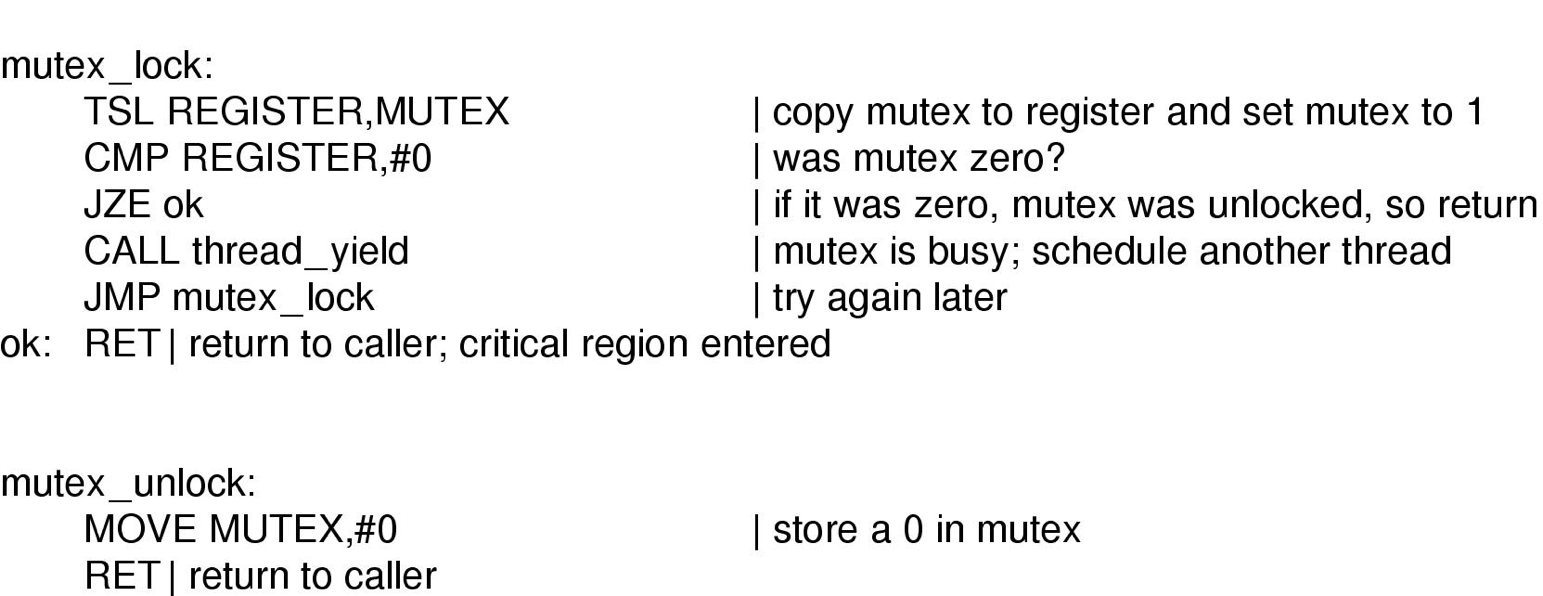
\includegraphics[scale=0.4]{m1/mutexWithTSL}
				\centering
			\end{figure}
			\begin{tcolorbox}
				\textsf{Problems with Semaphores: Deadlock} (on the left is the correct version)
				
				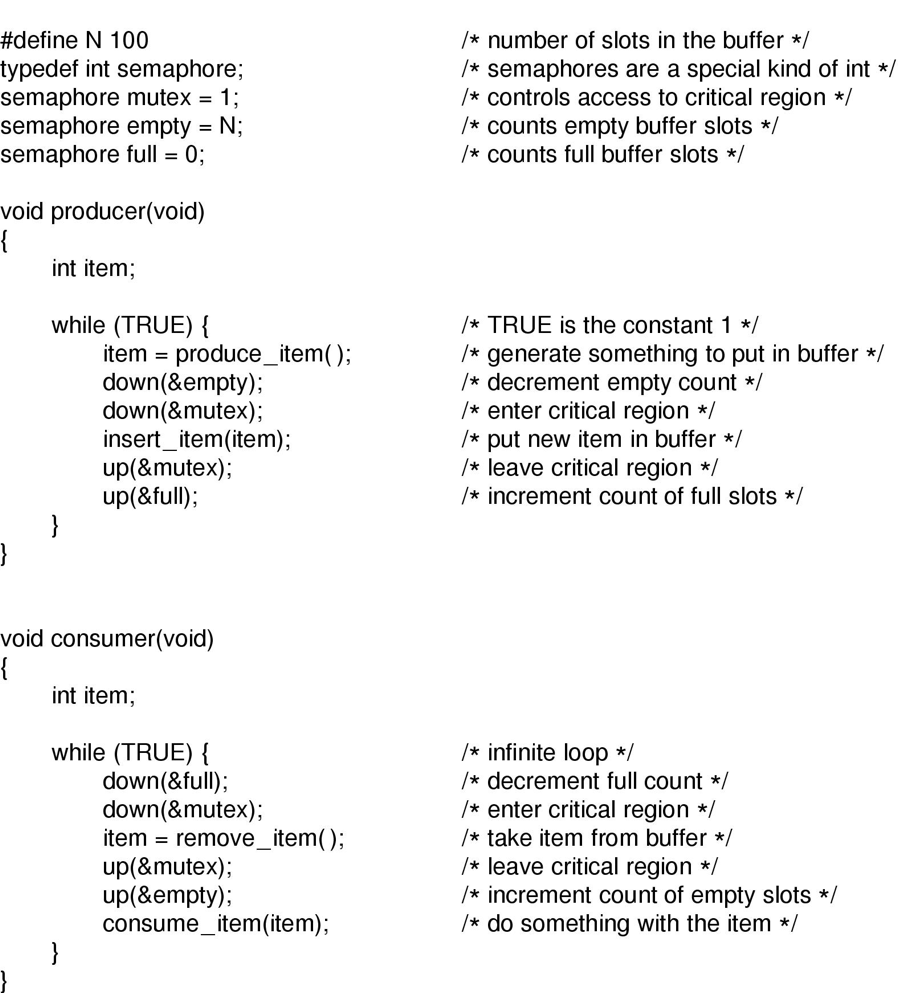
\includegraphics[scale=0.52]{m1/producerConsumerCode1}
				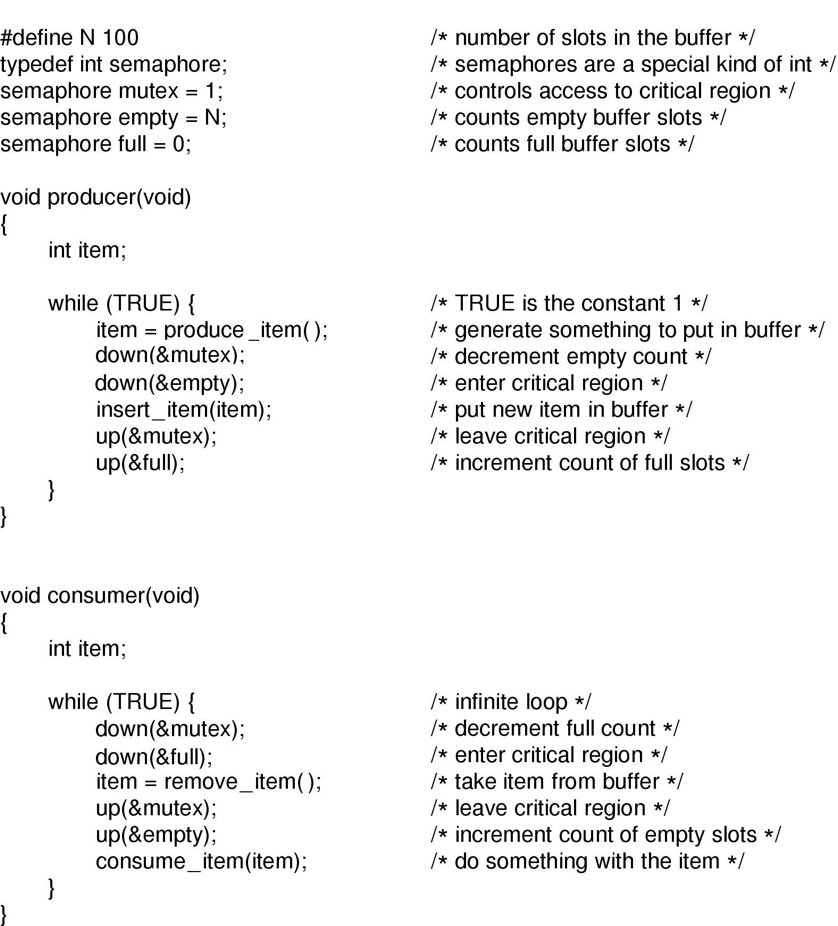
\includegraphics[scale=0.52]{m1/producerConsumerCode2}
				\centering
			\end{tcolorbox}
			\item Producer successfully DOWNs the mutex.
			\item Producer DOWNs “empty”. However the queue is full so this blocks.
			\item Consumer DOWNs mutex and blocks.
			\begin{myitemize}
				\item Consumer now never reaches the UP for “empty” and therefore cannot unblock the producer.
				\item The producer in turn never reaches the UP for mutex and cannot unblock the consumer. \textbf{Deadlock!}
			\end{myitemize}
			\begin{tcolorbox}
				\textsf{Reusable/Consumable Resources}
				\begin{myitemize}
					\item Reusable Resources - usually causes deadlocks
					\begin{myitemize}
						\item Examples: memory, devices, files, tables 
						\item Number of units is \textbf{constant}
						\item Unit is either free or allocated; \textbf{no sharing} (no simultaneous using) 
						\item Process \textbf{requests, acquires, releases units}
					\end{myitemize}
					\item Consumable Resources
					\begin{myitemize}
						\item Examples: messages, signals
						\item Number of units \textbf{varies} at runtime 
						\item Process \textbf{releases} (create) units (without acquire) 
						\item Other process \textbf{requests} and \textbf{acquires} (consumes)
						\item Deadlock when A and B are waiting for each other's message/ signal $\dots$
					\end{myitemize}
				\end{myitemize}
			\end{tcolorbox}
		\end{myitemize}
	\end{myitemize}
\end{example}

\begin{theorem}{\textbf{Dealing with deadlocks}}
	\begin{myenumerate}
		\item \textbf{Detection and Recovery}: Allow deadlock to happen and eliminate it
		\item \textbf{Avoidance (dynamic)}: Runtime checks disallow allocations that might lead to deadlocks
		\item \textbf{Prevention (static)}: Restrict type of request and acquisition to make deadlock impossible
	\end{myenumerate}
\end{theorem}

\begin{theorem}{\textbf{Conditions for Deadlock}}
	\begin{myenumerate}
		\item Mutual exclusion: Resources not sharable
		\item Hold and wait: Process must be \textbf{holding one} resource while \textbf{requesting another}
		\item Circular wait: \textbf{At least 2} processes must be blocked on each other
	\end{myenumerate}
\end{theorem}

\begin{method}{\textbf{Deadlock Prevention}}
	\begin{myenumerate}
		\item Eliminate mutual exclusion
		\begin{myitemize}
			\item Not possible in most cases
			\item Spooling makes I/O devices sharable
		\end{myitemize}
		\item Eliminate hold-and-wait 
		\begin{myitemize}
			\item \textbf{Request} all \textbf{resources at once}
			\item \textbf{Release} all resources \textbf{before a new request}
			\item \textbf{Release} all resources if \textbf{current request blocks}
		\end{myitemize}
		\item Eliminate circular wait
		\begin{myitemize}
			\item Order all resources
			\item Process must request in \textbf{ascending order}
		\end{myitemize}
	\end{myenumerate}
\end{method}

\begin{tcolorbox}
	\textsf{Problems with Semaphores: Priority Inversion}	priority(Process C) $<$ priority(Process B) $<$ priority(Process A), Process B effectively blocks out Process A, although Process A has higher priority!
	
	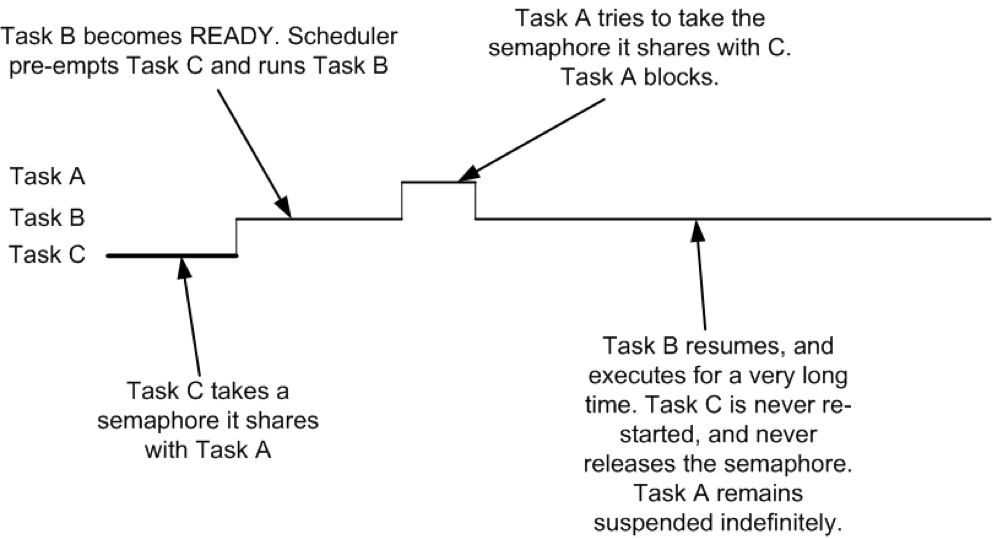
\includegraphics[scale=0.5]{m1/priorityInversion}
	\centering
\end{tcolorbox}

\begin{definition}{\textbf{Monitor}}, similar to a class or abstract-data type in C++ or JAVA:
	\begin{myitemize}
		\item \textbf{Collection of procedures}, variables and data structures grouped together in a package. Access to variables and data possible only through methods defined in the monitor.
		\item However, \textbf{only one} process can be active in a monitor at any point in time. I.e. if any other process tries to call a method within the monitor, it will block until the other process has exited the monitor.
		\item \textbf{Implementation}: (mutexes or binary semaphores)
		\begin{myitemize}
			\item When a process calls a monitor method, the method first checks to see if any other process is already using it. 
			\item If so, the calling process blocks until the other process has exited the monitor.
			\item The mutex/semaphore operations are inserted by the compiler itself rather than by the user, reducing the likelihood of errors.
		\end{myitemize}
	\end{myitemize}
\end{definition}

\begin{definition}{\textbf{Condition Variable} - mechanisms for coordination}
	\begin{myenumerate}
		\item One process WAITs on a condition variable and blocks.
		\item Another process SIGNALs on the same condition variable, unblocking the WAITing process.
	\end{myenumerate}
\end{definition}

\begin{tcolorbox}
	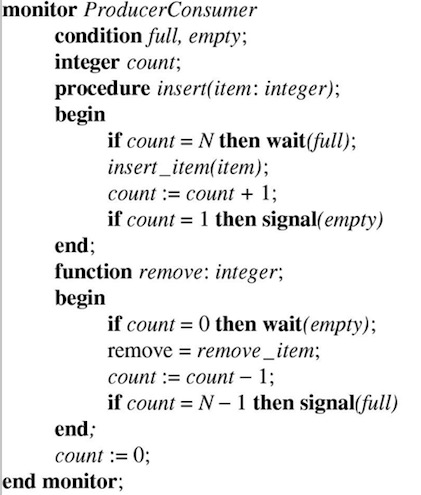
\includegraphics[scale=0.4]{m1/producerConsumerMonitor1}
	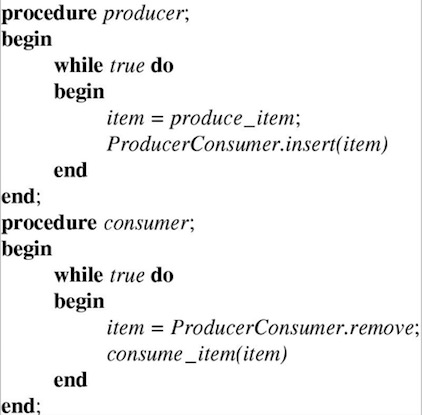
\includegraphics[scale=0.4]{m1/producerConsumerMonitor2}
	\centering	
	
	Similar to Sleep/Wake, however, the mutual exclusion from the monitor prevents the SIGNAL from being lost! 
\end{tcolorbox}

	\textsf{Monitors and Condition Variables Problems} - Violation of mutual exclusion
	\begin{myitemize}
		\item When a process encounters a WAIT, it is blocked and another process is allowed to enter the monitor.
		\item When there’s a SIGNAL, the sleeping process is woken up.
		\item We will potentially now have two processes in the monitor at the same time:
		\begin{myitemize}
			\item The process doing the SIGNAL (the signaler).
			\item The process that just woke up because of the SIGNAL (the signaled).
		\end{myitemize}
	\end{myitemize}

	\textsf{Ways to resolve}
	\begin{myitemize}
		\item We require that the signaler exits immediately after calling SIGNAL.
		\item We suspend the signaler immediately and resume the signaled process.
		\item We suspend the signaled process until the signaler exits, and resume the signaled process only after that.
	\end{myitemize}
	
\begin{remark}{\textbf{Comparison between semaphore and condition variable}}


	\noindent \textsf{Semaphore}
	\begin{myitemize}
		\item If Process A UPs a semaphore with no pending DOWN, the UP is saved.
		\item The next DOWN operation will not block because it will match immediately with a preceding UP.
	\end{myitemize}
	\textsf{Condition variable}
	\begin{myitemize}
		\item If Process A SIGNALs a condition variable with no pending WAIT, the SIGNAL is simply lost.
		\item This is similar to the SLEEP/WAKE problem earlier on.
	\end{myitemize}
\end{remark}

\begin{definition}{\textbf{Barrier}}
	is a special form of synchronization mechanism that works with groups of processes rather than single processes.
	\begin{center}
		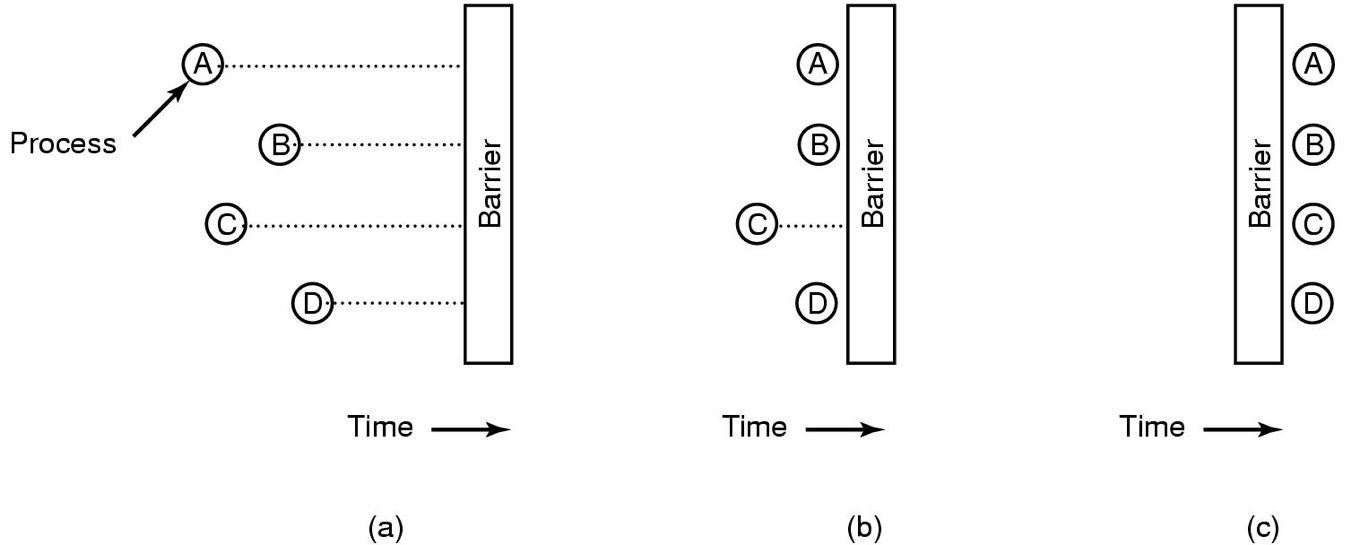
\includegraphics[scale=0.5]{m1/barrier}
	\end{center}
	
	The idea of a barrier is that all processes must reach the barrier (signifying the end of one phase of computation) before any of them are allowed to proceed.
	\begin{myitemize}
		\item Process D reaches the end of the current phase and calls a BARRIER primitive in the OS. It gets blocked.
		\item Similarly processes A and B reach the end of the current phase, calls the same BARRIER primitive and is blocked.
		\item Finally process C reaches the end of its computation, calls the BARRIER primitive, causing all processes to be unblocked at the same time.
	\end{myitemize}
\end{definition}

\begin{definition}{\textbf{UNIX Pipe}}
	\begin{myitemize}
		\item A pipe provides synchronisation
	\begin{myitemize}
		\item A process reading a pipe will block until there is data.
		\item Data send is asynchronous but blocks when buffer is full.
	\end{myitemize}
	\item A pipe provides byte-level message transfer between processes.
	\item Traditional method of communication between processes in UNIX: \textsf{Shell pipelines}
	\begin{myitemize}
		\item \textsf{grep buffer *.c $|$ sort -u $|$ wc}
		\item Output from program to left of bar provides input to program on right.
		\item Meaning: search for occurrences of string ''buffer'' in C files (grep process), sort those lines making them unique (sort process), and count how many occurrences  (wc process)
	\end{myitemize}
	\begin{center}
		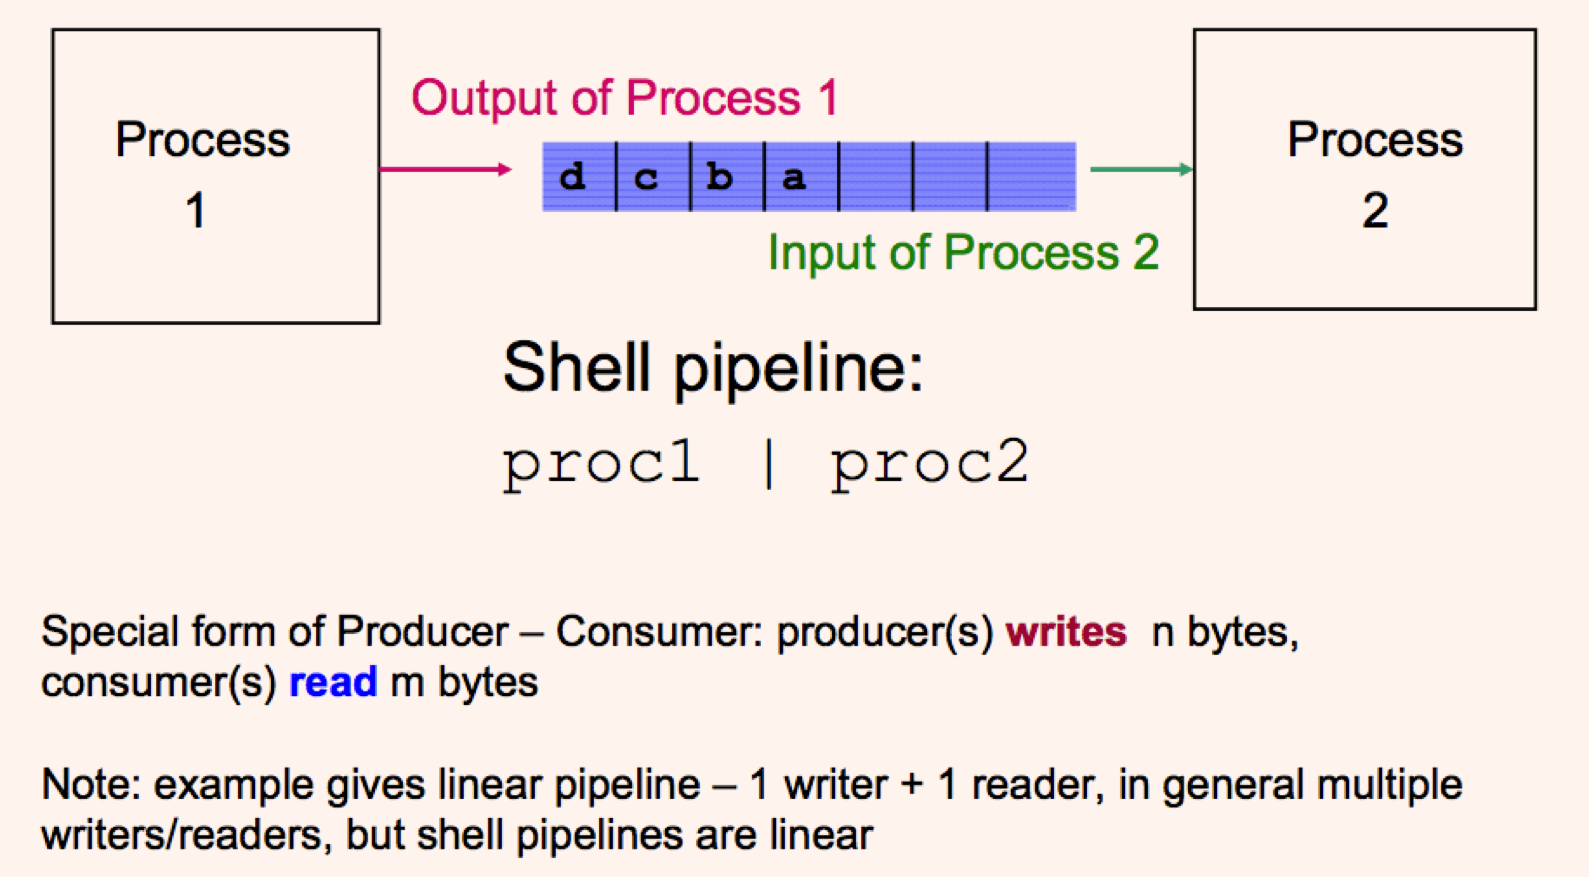
\includegraphics[scale=0.4]{m1/unixPipe}
	\end{center}
	\item Creating pipes: \textsf{int pipe(int fd\_array[])} returns 2 file descriptor for the (anonymous) pipe
	\begin{myitemize}
		\item Data is sent/received using normal write/read system calls
		\item write on \textsf{fd[1]}, read on \textsf{fd[0]}, e.g., \textsf{fd[1]} is the write end, \textsf{fd[0]} is the read end.
		\begin{center}
			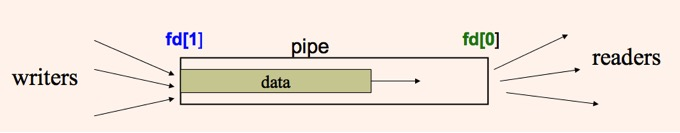
\includegraphics[scale=0.5]{m1/creatingPipe}
		\end{center}
		\item Some versions of Unix support duplex pipes, can readwrite on either end -- with corresponding write/read on opposite end; other Unixes only have one way pipes
		\item \textbf{File Descriptor}: a reference to a file when making system call, come from opening a file with \textsf{open()} system call but also other system calls which deal with files such as \textsf{pipe()}
	\end{myitemize}
	\end{myitemize}
\end{definition}
\begin{remark}
	\begin{myitemize}
		\item Closing unused pipe descriptor is good practice (not necessary to close all unused pipe descriptors).
		\item Closing the write end of the pipe, allows reader to determine when there is no more data: when all pipe ends closed, read gives EOF.
		\item Data read is the minimum of what is available and requested size. (e.g., \textsf{buffer} size is 100 but the string written was 10 chats)
		\item Pipes only used for unstructured byte streams.
	\end{myitemize}
\end{remark}

\begin{definition}{\textbf{FIFO files (Named pipes)}}
	\begin{myitemize}
		\item \textbf{Anonymous pipe}: can only use between related processes, e.g., parent + children.
		\item FIFO files are named pipes, pipes with a filename.
		\item Exist independent of process: any processes can use FIFO
		\item FIFO is a special file since it's really a pipe, cannot seek, no data is written to filesystem, every open FIFO corresponds to 1 pipe object.
		\item Can be created with \textsf{mkfifo} shell command or \textsf{mknod()} system call.
	\end{myitemize}
\end{definition}

\begin{example}{Shell named pipe}
	\begin{myenumerate}
		\item \textsf{mkfifo pipe; ls -l $>$ pipe}
		\item \textsf{cat pipe} (in another shell login)
	\end{myenumerate}
\end{example}

\begin{example}{Programming named pipe}

\noindent\begin{minipage}{.48\textwidth}
\begin{lstlisting}[caption=writer.c,frame=tlrb,language=C]{Name}
    int fd;
    char * myfifo = "/tmp/myfifo";

    mkfifo(myfifo, 0666);

    fd = open(myfifo, O_WRONLY);
    write(fd, "Hi", sizeof("Hi"));
    close(fd);

    /* remove the FIFO */
    unlink(myfifo);
\end{lstlisting}
\end{minipage}\hfill
\begin{minipage}{.48\textwidth}
\begin{lstlisting}[caption=reader.c,frame=tlrb,language=C]{Name}
    int fd;
    char * myfifo = "/tmp/myfifo";
    char buf[MAX_BUF];

    /* open, read, and display */
    fd = open(myfifo, O_RDONLY);
    read(fd, buf, MAX_BUF);
    printf("Received: %s\n", buf);
    close(fd);

\end{lstlisting}
\end{minipage}
\textbf{Note}: When only one program is run it will hang. writer.c blocks at the ''write'' statement, which means it will not call unlink to delete the named pipe until the reader has read the pipe.

\end{example}


% $$$$$$$$$$$$$$$$$$$$$$$$$$$$$$$$$$ %

\end{document}